%\documentclass[12pt]{book}
\documentclass[10pt]{article}
\usepackage{color,amsmath}
\usepackage{verbatim}
\usepackage{multirow} 
\usepackage{draftwatermark}
\SetWatermarkLightness{0.8}
\SetWatermarkScale{5}

% ===    Set a true/false value for PDF hyper marks  

\newif\ifhyprf
%\hyprffalse
\hyprftrue
    
\RequirePackage{ifpdf}

\ifpdf
    \pdfoutput=1        % we are running PDFLaTeX
    \pdftrue
\else
    \pdffalse           % we are not running PDFLaTeX
\fi

\ifpdf
  \pdfcompresslevel=9
  \usepackage[pdftex]{graphicx}
%  \usepackage{thumbpdf}
  \definecolor{rltred}{rgb}{0.75,0,0}
  \definecolor{rltgreen}{rgb}{0,0.3,0}
  \definecolor{rltblue}{rgb}{0,0,0.75}
  \definecolor{rltdarkgreen}{rgb}{0.1,0.6,0.1}
  \ifhyprf
     \usepackage[pdftex,
         colorlinks=true,
         urlcolor=rltblue,       % \href{...}{...} external (URL)
         filecolor=rltgreen,     % \href{...} local file
         linkcolor=rltred,       % \ref{...} and \pageref{...}
         citecolor=rltdarkgreen, % citations
         pagebackref,
         pdfpagemode=None,
         pdftitle={BDX: on-beam background assess and MC validation},
         pdfauthor={many},
         pdfsubject={Beam dump experiment JLab Hall A},
         pdfkeywords={Hall A, Beam dump, dark photon}]{hyperref}
  \fi
  \usepackage{pdfcolmk}
  \DeclareGraphicsExtensions{.pdf,.png,.jpg}
\else
  \usepackage{graphicx}
  \DeclareGraphicsExtensions{.eps,.epsi,.ps,.eps.gz,.epsi.gz,.ps.gz}
\fi

\setlength{\textwidth}{6.0in}
%\setlength{\textheight}{9.5in}
\setlength{\textheight}{8.0in}
\setlength{\evensidemargin}{0.25in}
\setlength{\oddsidemargin}{0.25in}
\setlength{\topmargin}{-0.25in}
\setlength{\footskip}{0.25in}
%\setlength{\parindent}{0pt}
%\setlength{\parskip}{0in}
\usepackage{graphicx,lscape,rotating}
\pagenumbering{arabic}
%\input epsf

\usepackage{amsmath}
\usepackage{amssymb,amsfonts,textcomp}

% The package lineno adds line numbers to LaTeX documents.
\usepackage{lineno}


%%%%%%%%
%%%%%%%%
\newcommand{\fb}{{\rm fb}}
\newcommand{\ab}{{\rm ab}}

\newcommand{\be}{\begin{eqnarray}}
\newcommand{\ee}{\end{eqnarray}}
\def\lsim{\mathrel{\rlap{\lower4pt\hbox{\hskip 0.5 pt$\sim$}}
\raise1pt\hbox{$<$}}}                % less than or approx. symbol
\def\gsim{\mathrel{\rlap{\lower4pt\hbox{\hskip1pt$\sim$}}
\raise1pt\hbox{$>$}}}

\newcommand{\schi}{s_{\chi\bar\chi}}  % tried to use this throughout off-shell derivation so that we can change notation later if desired.
\newcommand{\scratch}[1]{{\textcolor{red}{ #1}}}
\newcommand{\f}{\frac}
\newcommand{\pf}[2]{\left(\frac{#1}{#2}\right)}
\newcommand{\g}{{\rm g}}
\newcommand{\s}{{\rm s}}
\newcommand{\m}{{\rm m}}
\newcommand{\apr}{{A^\prime}}
\newcommand{\MeV}{{\rm MeV}}
\newcommand{\GeV}{{\rm GeV}}


\makeatletter
\newcommand\arraybslash{\let\\\@arraycr}
\makeatother
\setlength\tabcolsep{1mm}
\renewcommand\arraystretch{1.4}

\newcommand{\thedate}{\today}

\renewcommand{\thefootnote}{\fnsymbol{footnote}}


%%%%%%%%
%%%%%%%%





\newcommand{\la}{\langle}
\newcommand{\ra}{\rangle}
\newcommand{\zh}{z}
\newcommand{\xbj}{x_{\scriptscriptstyle B}}
%
\newcommand{\thp}{$\Theta^+$ }
\newcommand{\Thgg}{$\theta_{\gamma^*\gamma}~$}
\newcommand{\Phgg}{$\phi_{\gamma^*\gamma}~$}
\newcommand{\Epg}{$ep~\rightarrow~ep\gamma~$}
\newcommand{\Eppiz}{$ep~\rightarrow~ep\pi^0~$}
\newcommand{\Enpip}{$ep~\rightarrow~en\pi^+~$}
\newcommand{\EppiD}{$ep~\rightarrow~e\pi \Delta~$}
\newcommand{\Epeta}{$ep~\rightarrow~ep\eta~$}
\newcommand{\Epr}{$ep~\rightarrow~ep\rho~$}
\newcommand{\EpX}{$ep~\rightarrow~epX~$}
\newcommand{\EpKY}{$ep~\rightarrow~eKY~$}
\newcommand{\vEpg}{$\vec ep~\rightarrow~ep\gamma~$}
\def\gevc2{(GeV/c)$^2$}
\newcommand*{\jlab}{Jefferson Lab, Newport News, VA 23606, USA}
\newcommand*{\nhs}{University of New Hampshire, Durham NH 03824, USA}
\newcommand*{\perimeter}{Perimeter Institute for Theoretical Physics, Waterloo, Ontario, Canada, N2L 2Y5}
\newcommand*{\yerevan}{Yerevan Physics Institute, 375036 Yerevan, Armenia}
\newcommand*{\frascati}{Istituto Nazionale di Fisica Nucleare, Laboratori Nazionali di Frascati, P.O. 13, 00044 Frascati, Italy}
\newcommand*{\genova}{Istituto Nazionale di Fisica Nucleare, Sezione di Genova, 16146 Genova, Italy}
\newcommand*{\sanita}{Istituto Nazionale di Fisica Nucleare, Sezione di Roma e Gruppo Collegato Sanit\`a,
 e  Universit\`a La Sapienza, Italy}
\newcommand*{\infnct}{Istituto Nazionale di Fisica Nucleare, Sezione di Catania e Dipartimento di Fisica dell'Universit\`a, Catania, Italy}
\newcommand*{\infnba}{Istituto Nazionale di Fisica Nucleare, Sezione di Bari e Dipartimento di Fisica dell'Universit\`a, Bari, Italy}
\newcommand*{\infnfe}{Istituto Nazionale di Fisica Nucleare, Sezione di Ferrara e Dipartimento di Fisica dell'Universit\`a, Ferrara, Italy}
\newcommand*{\infnle}{Istituto Nazionale di Fisica Nucleare, Sezione di Lecce 73100 Lecce, Italy}
\newcommand*{\saclay}{CEA-Saclay, Service de Physique Nucleaire, F91191 Gif-sur-Yvette, France}

\newcommand*{\ipn}{Institut de Physique Nucleaire d'Orsay, IN2P3, BP 1, 91406 Orsay, France}
\newcommand*{\grenoble}{Laboratoire de Physique et de Cosmologie, CNRS/IN2P3, 38026 Grenoble, France}
\newcommand*{\isu}{Idaho State University, Department of Physics, Pocatello, Idaho 83209}
\newcommand*{\uvch}{University of Virginia, Department of Physics, Charlottesville, VA 22903, USA}
\newcommand*{\nsuva}{Norfolk State University, Norfolk VA 23504, USA}
\newcommand*{\rpi}{Rensselaer Polytechnic Institute, Department of Physics, Troy, NY 12181, USA}
\newcommand*{\moscow}{Moscow  State University, 119899 Moscow, Russia}
\newcommand*{\ucla}{University of California at Los Angeles, Department of Physics and 
Astronomy, Los Angeles, CA 90095-1547, USA}
\newcommand*{\ohio}{Ohio University, Department of Physics, Athens, OH 45701, USA}
\newcommand*{\gwu} {The George Washington University, Washington, D.C., 20052}
\newcommand*{\cua} {
Catholic University of America, Washington, D.C. 20064}
\newcommand*{\odu}{Old Dominion University, Department of Physics,
Norfolk VA 23529, USA}
\newcommand*{\unh}{University of New Hampshire, Department of
Physics, Durham, NH 03824, USA}
\newcommand*{\cudc}{Catholic University of America, Department of Physics, Washington D.C., 20064, USA}
\newcommand*{\ucon}{University of Connecticut, Physics Department, Storr, CT 06269, USA}
\newcommand*{\edinb}{Edinburgh University, Edinburgh EH9 3JZ, United Kingdom}
\newcommand*{\glasgow}{University of Glasgow, Glasgow G12 8QQ, United Kingdom}
\newcommand*{\iu}{Physics Department and Nuclear Theory Center, Indiana University, Bloomington, Indiana 47405}
\newcommand*{\lanl}{Los Alamos National Laboratory, New Mexico, NM}
\newcommand*{\ASU}{Arizona State University, Tempe, Arizona 85287-1504}
\newcommand*{\uconn}{University of Connecticut, Storrs, Connecticut 06269}
\newcommand*{\fiu}{Florida International University, Miami, Florida 33199}
\newcommand*{\jmu}{James Madison University, Harrisonburg, Virginia 22807}
\newcommand*{\utfsm}{Universidad T\'ecnica Federico Santa Mar\'ia, Valpara\'iso, Chile}
\newcommand{\sassari}{Universit\`a di Sassari e Istituto Nazionale di Fisica Nucleare, 07100 Sassari, Italy}
\newcommand{\torvergata} {Istituto Nazionale di Fisica Nucleare, Sezione di Roma-TorVergata e Dipartimento di Fisica dell'Universit\`a, Roma, Italy}
\newcommand{\catania} {Istituto Nazionale di Fisica Nucleare, Sezione di Catania,  Catania, Italy}
\newcommand{\torino} {Istituto Nazionale di Fisica Nucleare, Sezione di Torino,  Torino, Italy}
\newcommand{\padova} {Istituto Nazionale di Fisica Nucleare, Sezione di Padova,  Padova, Italy}
\newcommand*{\hu}{Department of Physics, Hampton University, Hampton VA 23668, USA }
\newcommand*{\canisius}{Canisius College, Buffalo NY 14208, USA}
\newcommand*{\occidental}{Occidental College, Los Angeles, California 90041, USA}
\newcommand*{\unm}{University of New Mexico, Albuquerque, New Mexico, NM}
\newcommand*{\mainz}{Institut fur Kernphysik, Johannes Gutenberg-Universitat Mainz, 55128 Mainz, Germany}
\newcommand*{\slac}{Stanford Linear Accelerator Center (SLAC), Menlo Park, CA 94025, US}
\newcommand*{\fnal}{Center for Particle Astrophysics, Fermi National Accelerator Laboratory, Batavia, IL 60510}
\newcommand*{\msu}{Mississippi State University, Mississippi State, MS 39762, USA}
\newcommand*{\stony}{C.N. Yang Inst. for Theoretical Physics, Stony Brook University, NY}
\newcommand*{\idaho}{Dept. of Physics, Idaho State University, Pocatello, ID 83201  USA}
\newcommand*{\spaolo}{Instituto de Fisica, Universidade de S\~ao Paulo, Brasil}
\newcommand*{\northw}{Northwestern University, Evanston, IL 60208, USA}
\newcommand*{\julich}{Nuclear Physics Institute and Juelich Center for Hadron Physics, Forschungszentrum Juelich, Germany}
\newcommand*{\mito}{Massachusetts Institute of Technology, Cambridge, MA 02139, USA}











% this extends the number of footnote symbols allowed

\usepackage{alphalph}
\makeatletter
\newcommand*{\fnsymbolsingle}[1]{%
\ensuremath{%
\ifcase#1%
\or *%
\or \dagger
\or \ddagger
\or \mathsection
\or \mathparagraph
\else
\@ctrerr \fi
}%
}
\makeatother
\newalphalph{\fnsymbolmult}[mult]{\fnsymbolsingle}{}
\renewcommand*{\thefootnote}{%
\fnsymbolmult{\value{footnote}}%
}



%
%%%%%%%%%%%%%%%%%%%%%%%%%%%%%%%%%%%%%%%%%%%%%%%%%%%%%%
%

\begin{document}

\begin{center}
{\tiny \leftline{V0.0}}
{\tiny\leftline{\thedate}}
\date{\today}
%\rightline{***DRAFT*** Proposal to PAC 44}
\vskip 1.0cm
{\bf\huge BDX on-beam background assess and MC validation}

\vskip 0.5cm

{ M.~Battaglieri, A.~Celentano, R.~De~Vita,L.~Marsicano\\}
{\small\it\genova}
\vskip 0.2cm
{ M.~Bond\'i, M.~De Napoli, N.~Randazzo\\}
{\small\it\catania\\}
\vskip 0.2cm
{G. Kharashvili, E.S.~Smith\\}
{\it\small\jlab}
\vskip 0.2cm
{E. Izaguirre\\}
{\small\it\perimeter}
\vskip 0.2cm
{G. Krnjaic\\}
{\small\it\fnal}
\vskip 0.2cm
{D.~Snowden-Ifft\\}
{\it\small\occidental}
\vskip 0.2cm
{M.~Carpinelli, V.~Sipala\\}
{\small\it\sassari}
\vskip 0.5cm
{\it and The BDX Collaboration }

\begin{abstract}
\textcolor{red} {}
In response to the issue raised by JLAB-PAC44  about the experiment proposal  {\it PR-16-001 Dark matter search in a Beam-Dump eXperiment (BDX) at Jefferson Lab}~\cite{vdx-proposal} we propose to measure  the prompt  radiation  produced by the interaction of the high intensity 11 GeV electron beam with the Hall-A beam dump. The muon and neutron  flux will be sampled at different height (with-respect-to the beam line), positions  and angles downstream of the beam dump to map out the radiation field in the location of the  future hall hosting the BDX experiment. In order to realistically assess the beam-on background experienced by the BDX detector, 
 a specimen of the CsI(Tl) crystal from the  BDX electromagnetic calorimeter, will be exposed to the radiation as part of a plastic scintillator hodoscope built  specifically for this measurement (BDX-Hodo). Although it will not be possible to directly compare results of this tests with the experimental set up proposed in PR-16-001 that will make use of a different and  optimised shielding, the measurement will be extremely useful to validate the MonteCarlo simulation tools (GEANT4 and FLUKA) used to design the new underground facility and optimize the BDX detector.

This report is organised as follow: 
results of the simulation of the radiation field produced by the interaction of the beam with the dump  are reported in Sec.~\ref{sec: sim}; 
the experimental set-up and the detector is described in Sec.\ref{sec:setup}; the expected results of the measurement are reported in Sec.~\ref{sec: results}. Details about cost estimate to run the test, work -and time-planes are reported in the Appendix.

\end{abstract}

\vskip 1.0cm
 
\end{center} 

%\newpage
\tableofcontents
\newpage


%\linenumbers

\section{MC simulations}
\label{sec:sim}
\subsection{The Hall-A high-power beam-dump}
The Hall A and C use identical high-power absorbing (up to 1 MW)  beam-dumps to stop the 11 GeV beam, remnant of beam/target interaction. The dump is made by a set of about 80 aluminium disks, each
approximately 40 cm in diameter of increasing thickness (from 1 to 2 cm), for a total
length of approximately 200 cm, followed by a solid Al cylinder 50 cm in diameter
and approximately 100 cm long. They are both cooled by circulating water. The full
drawing of the beam-dump is shown in Fig.~\ref{fig:bd}. To increase the radiation shielding,
the thickness of the concrete tunnel surrounding the Al dump is about 4-5 m thick.

\begin{figure}[h!] 
\center
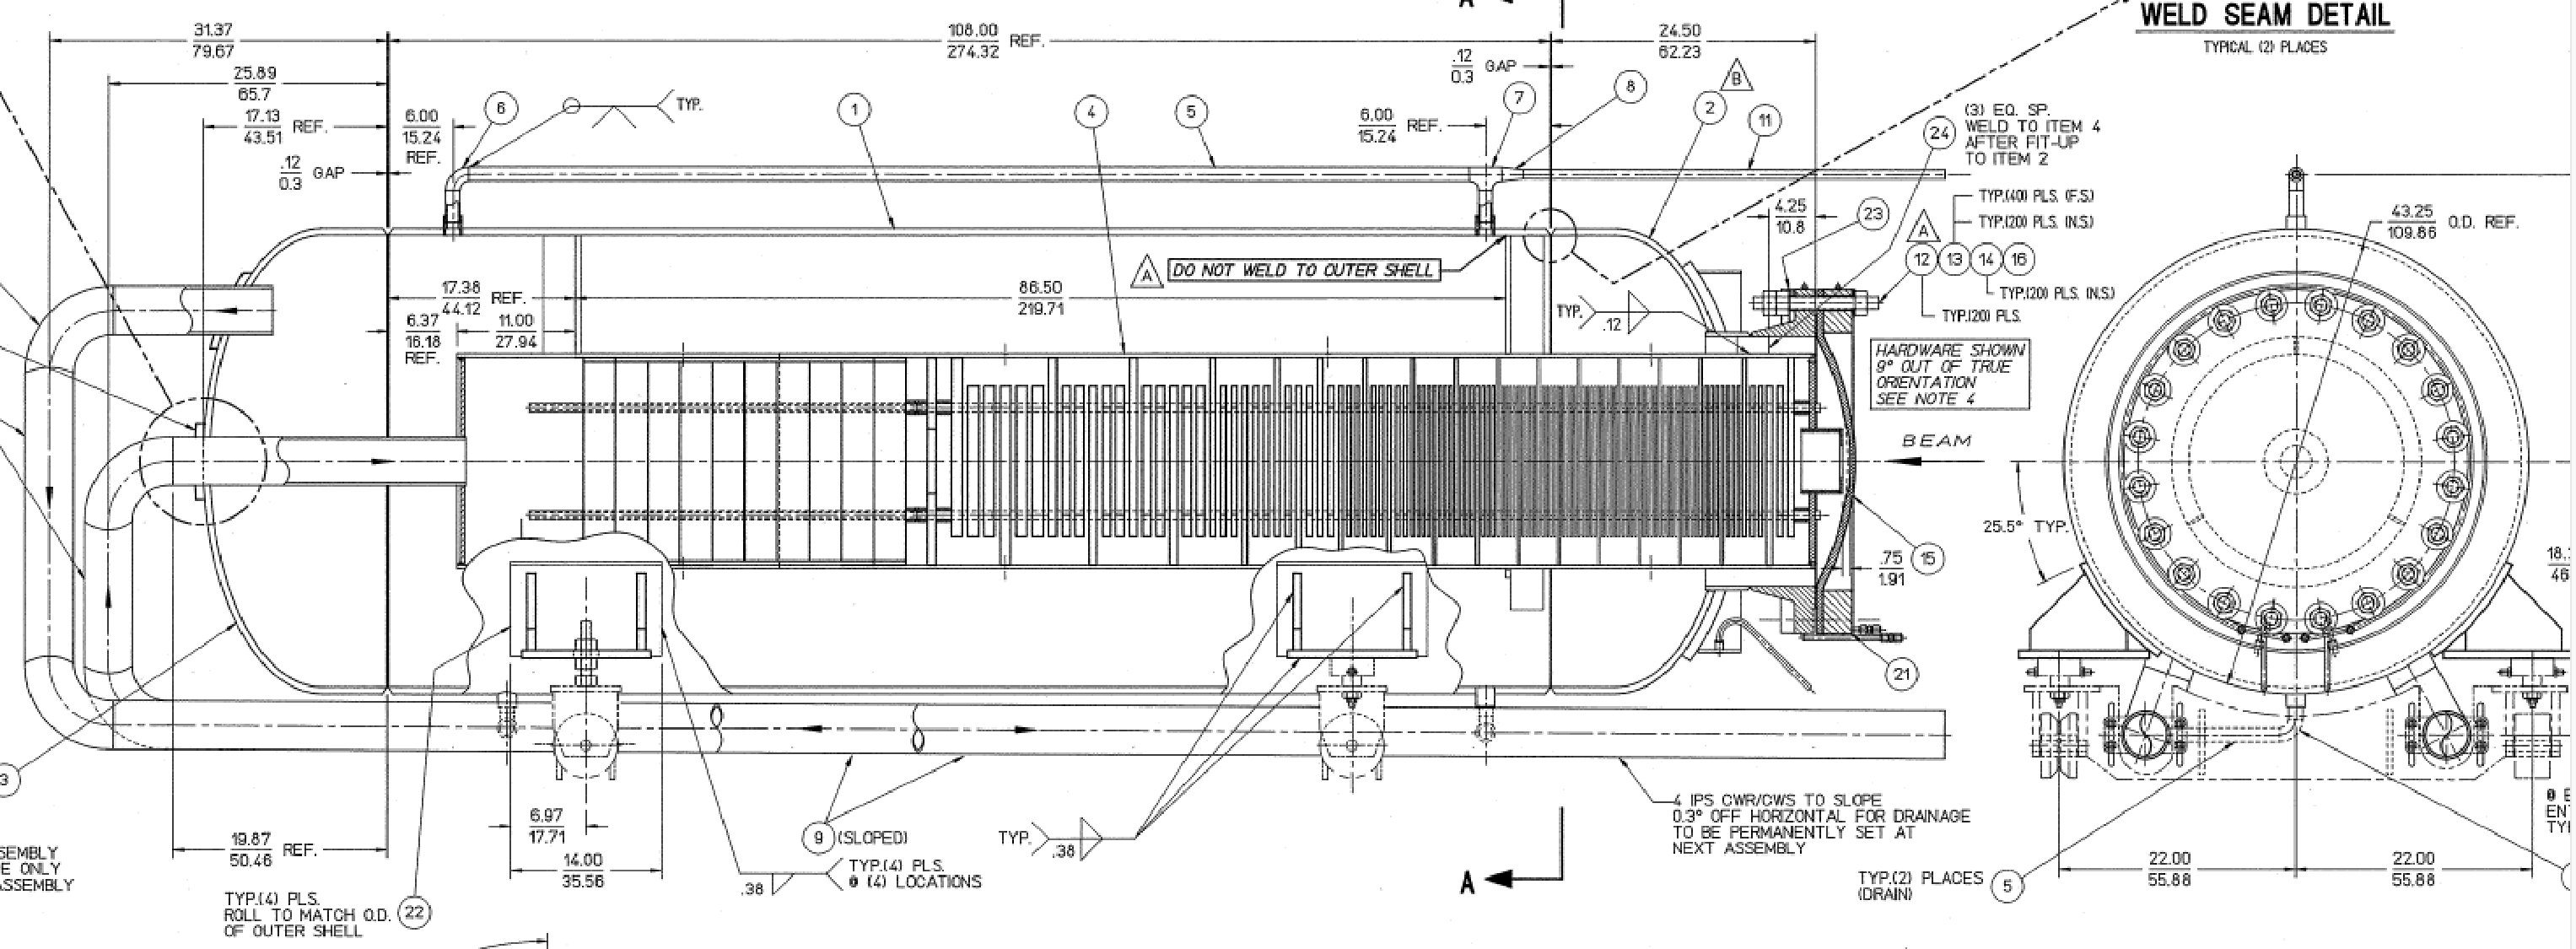
\includegraphics[width=12.5cm]{figs/beam-dump-br.pdf}
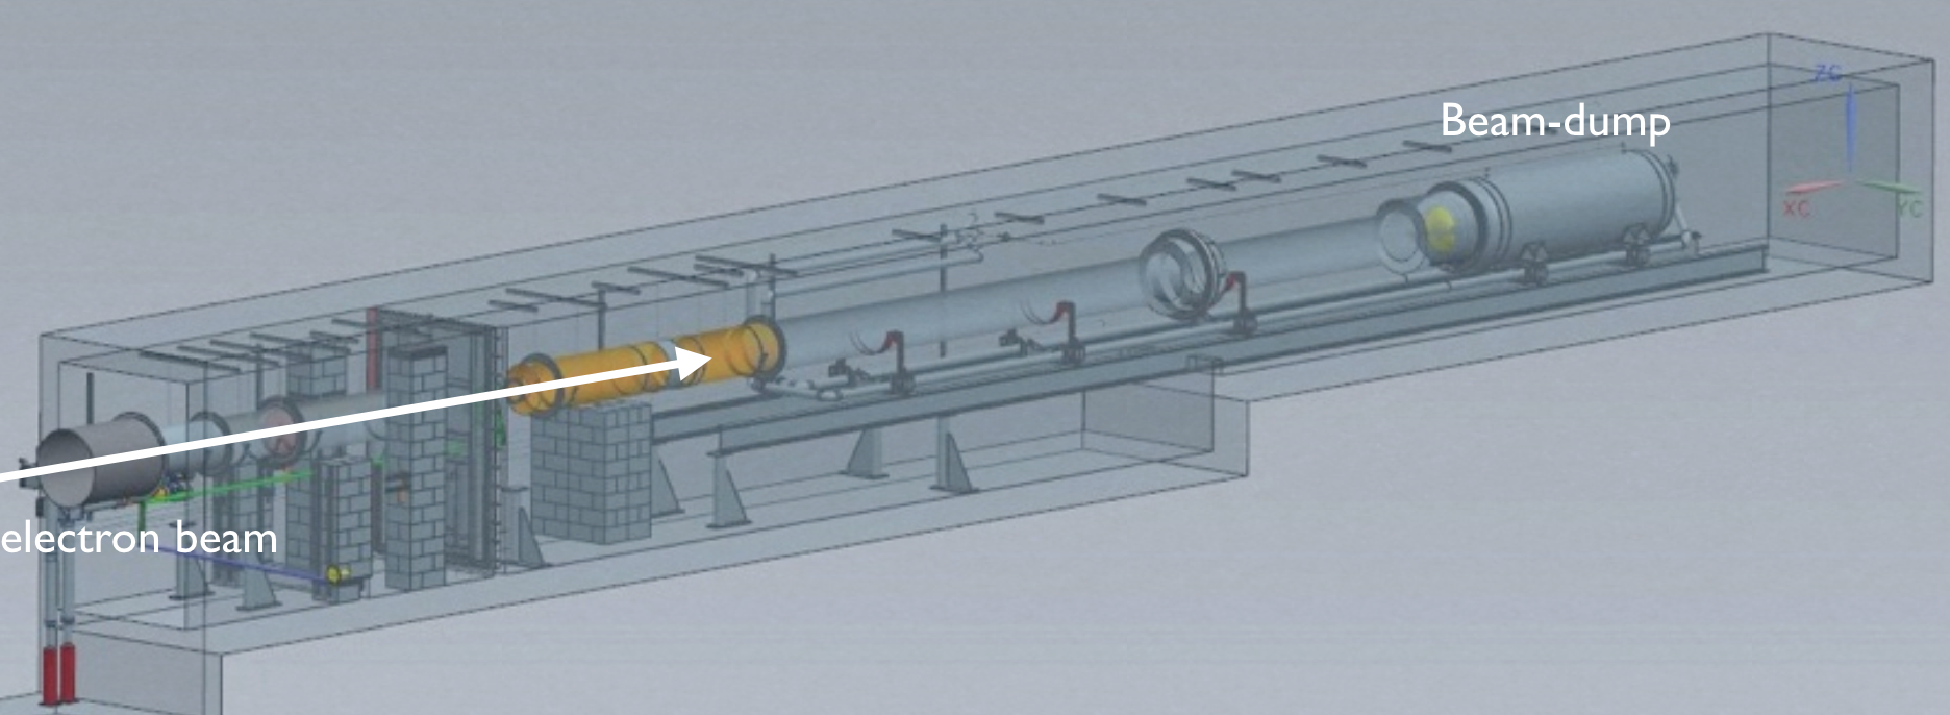
\includegraphics[width=12.5cm]{figs/beam-dump.pdf}
\caption{Hall-A beam dump and beam dump enclosure. }
\label{fig:bd}
\end{figure}
\begin{figure}[h!] 
\center
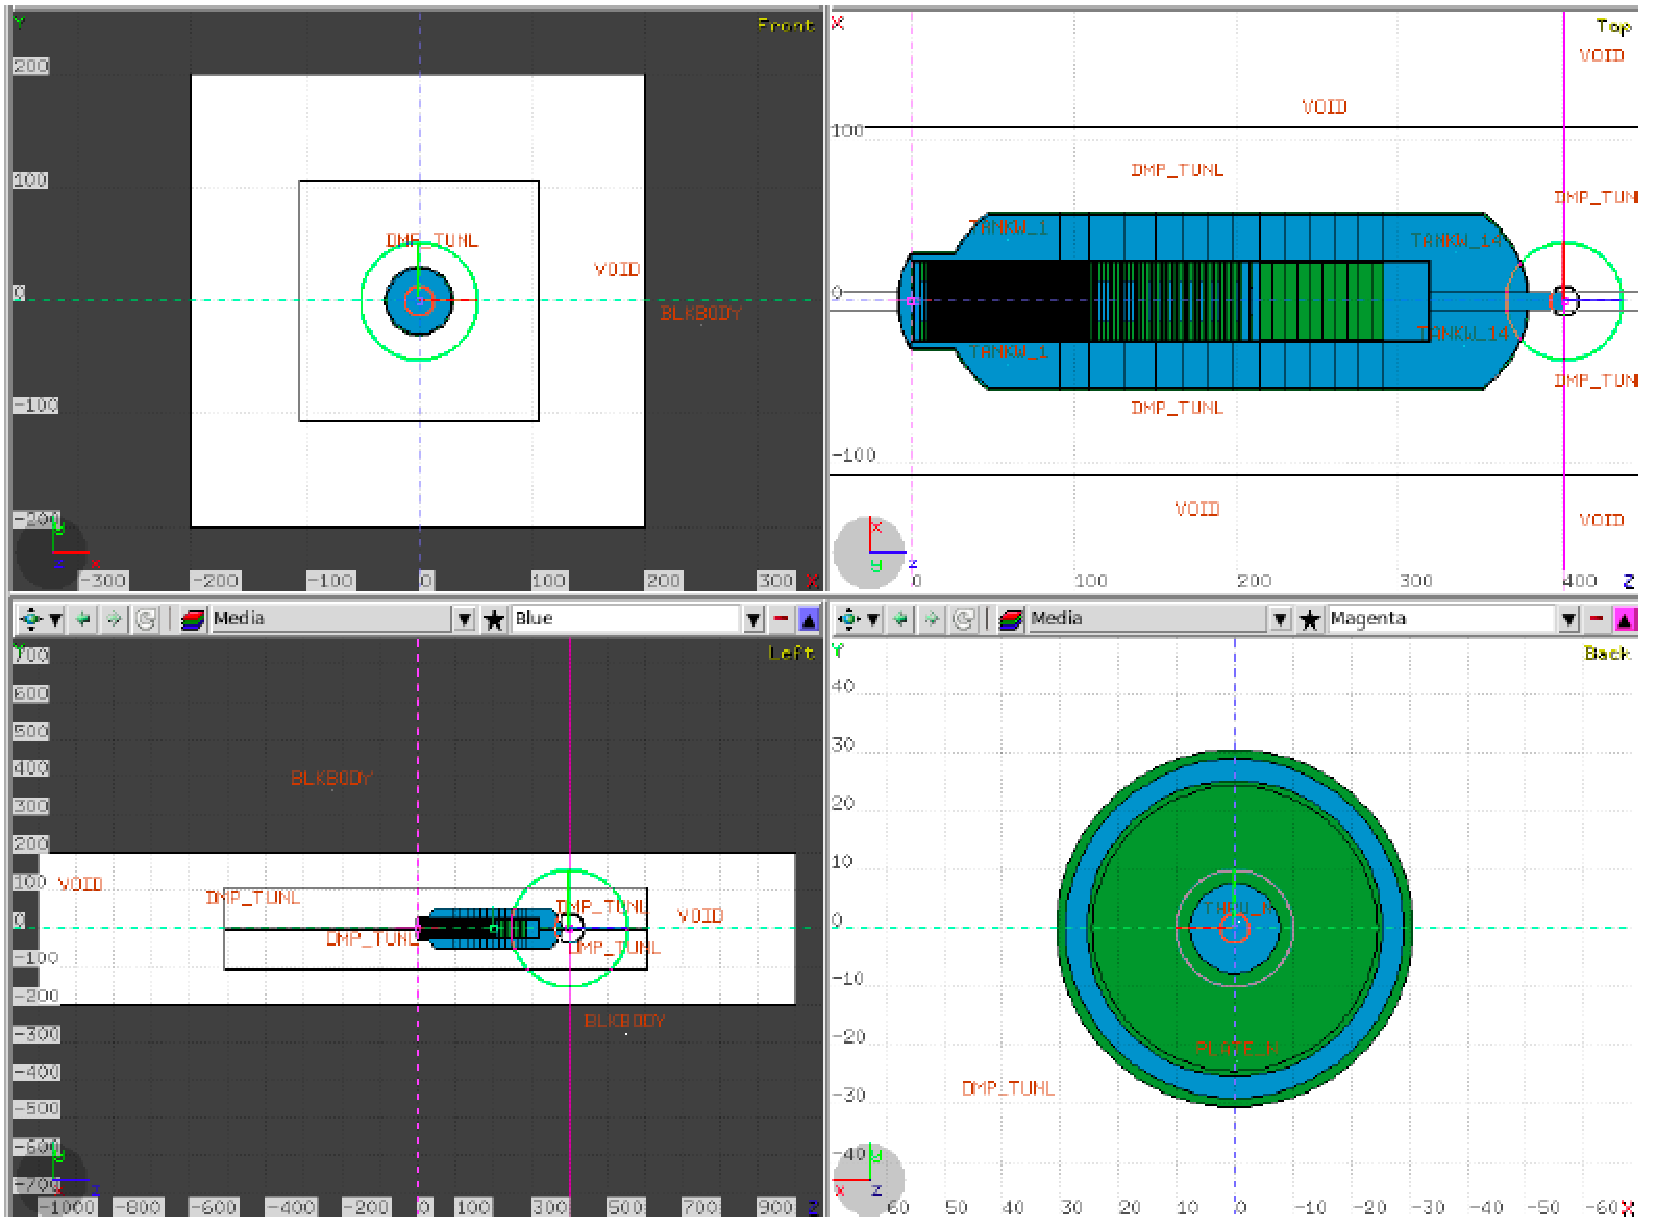
\includegraphics[width=14.5cm]{figs/fluka-bd.pdf}
\caption{Hall-A beam-dump implementation in FLUKA. }
\label{fig:fluka-bd}
\end{figure}
\begin{figure}[h!] 
\center
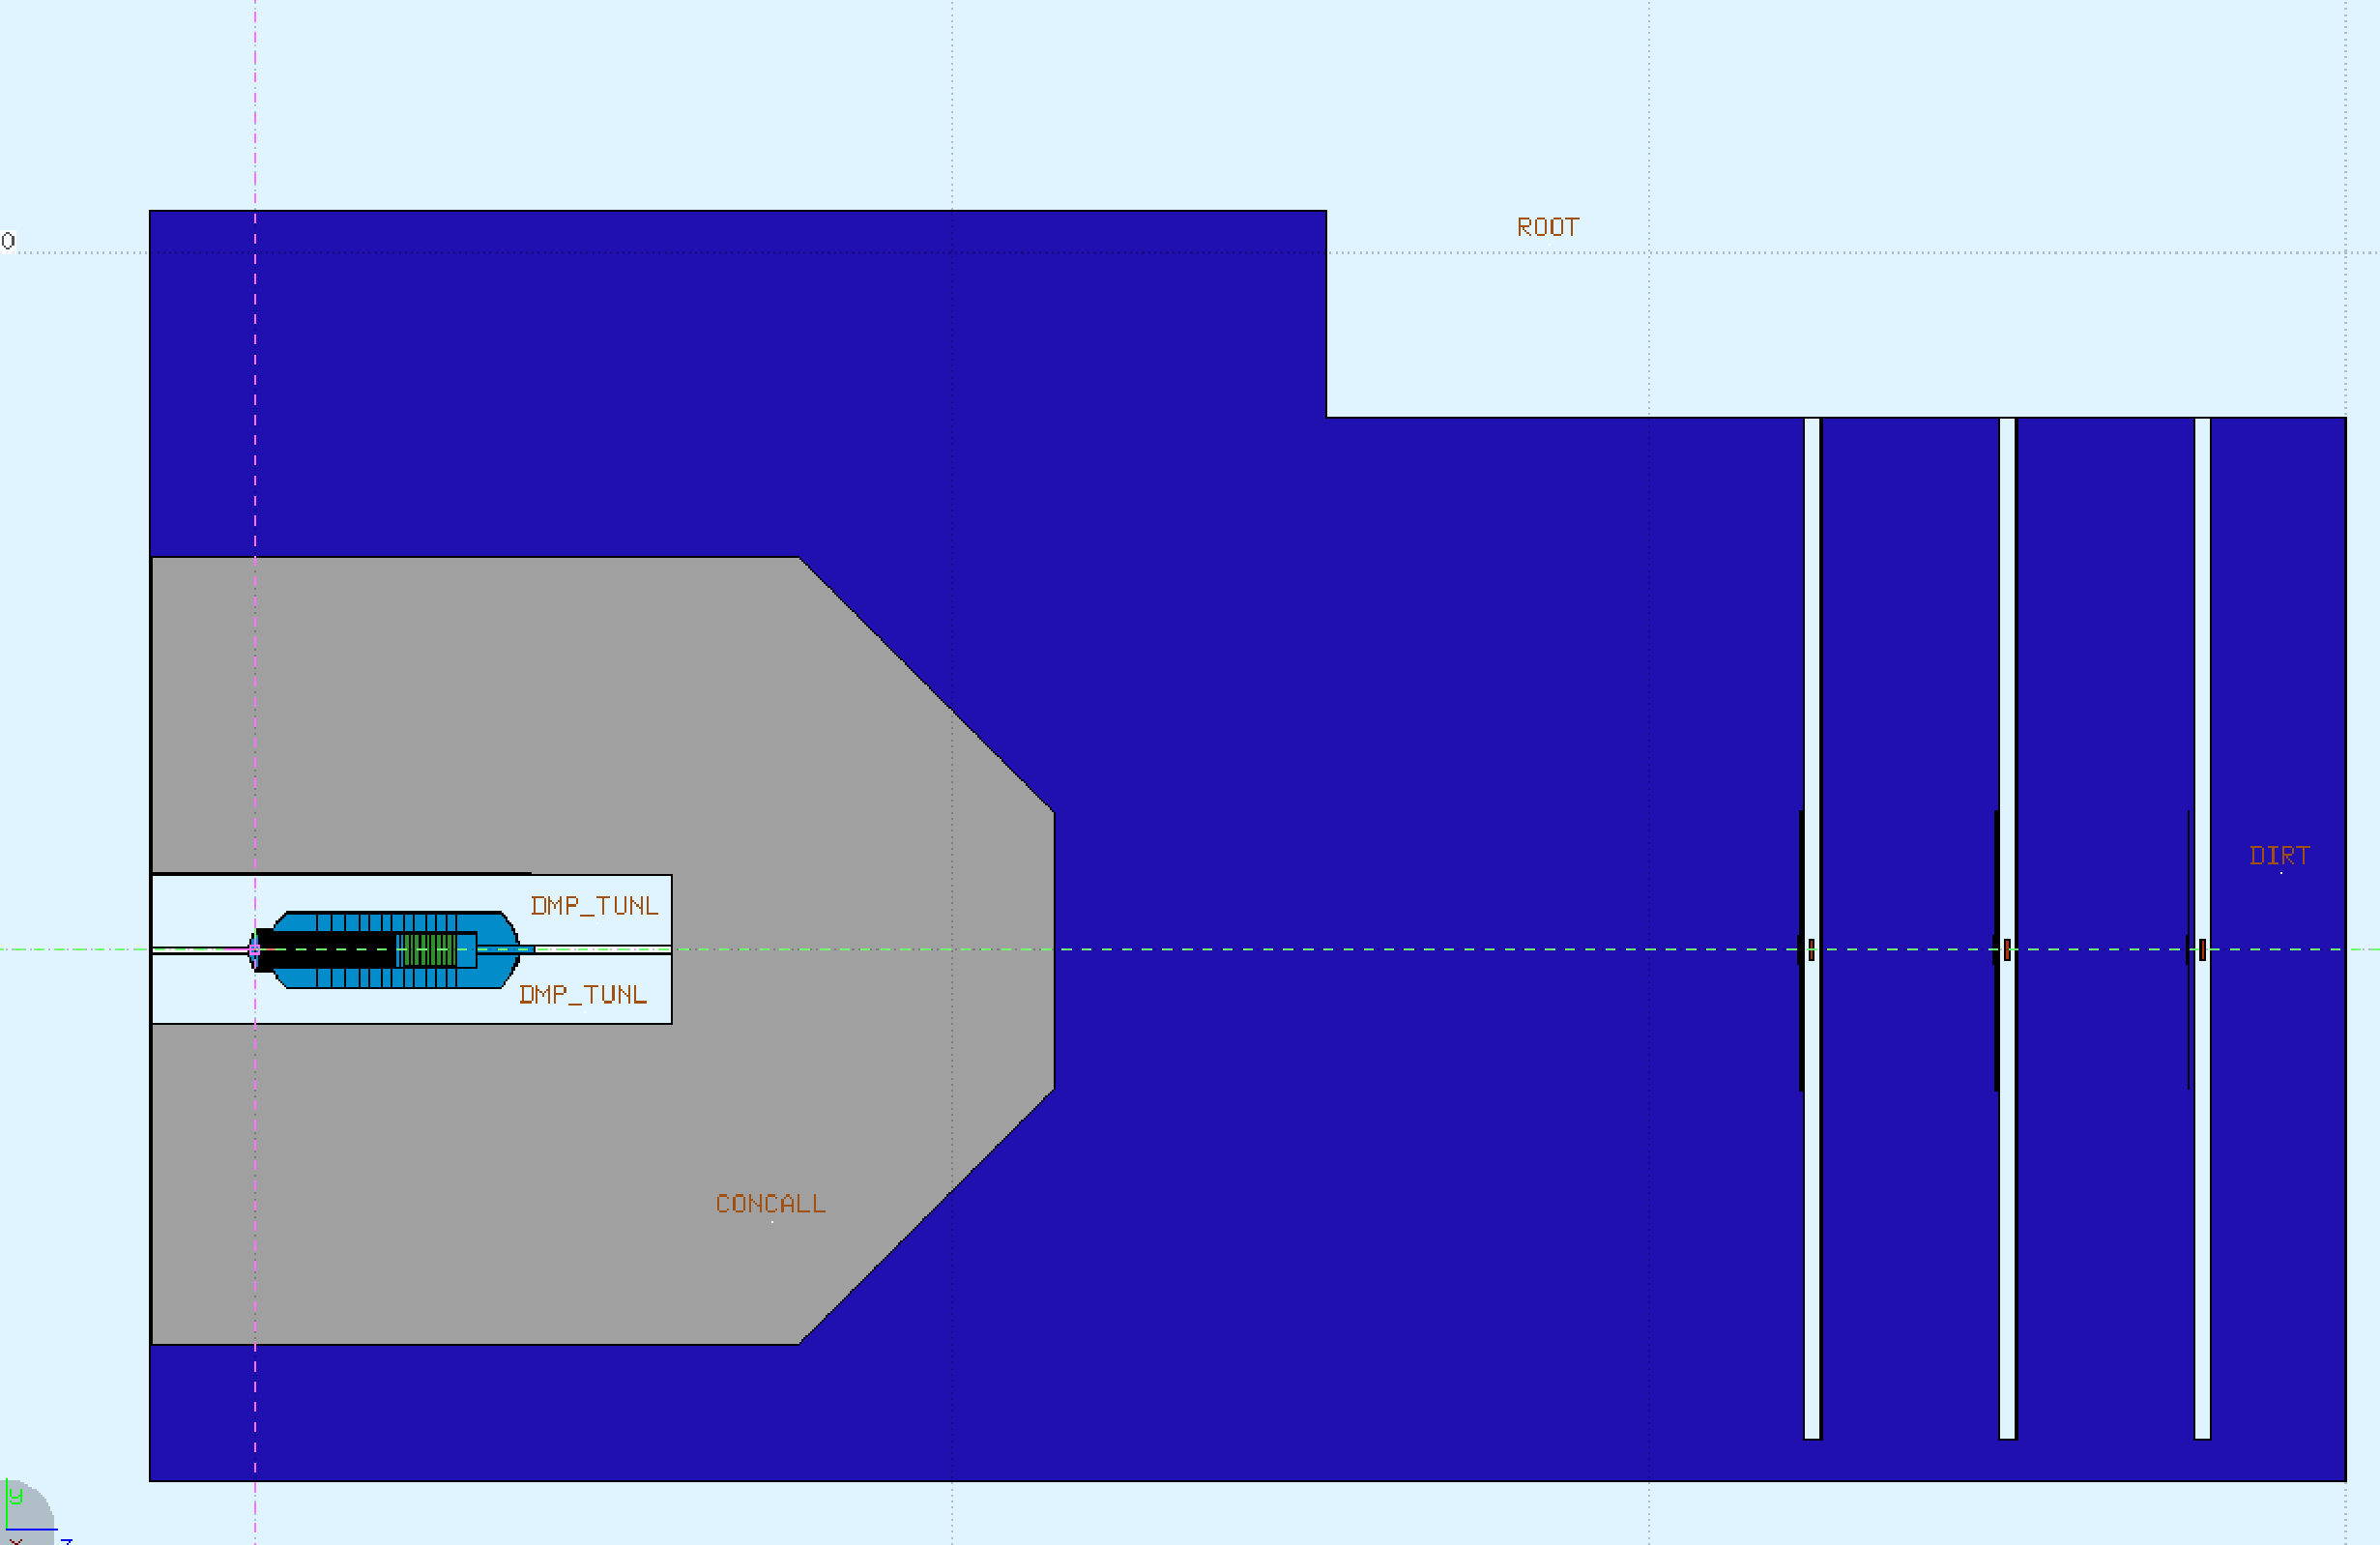
\includegraphics[width=12.5cm]{figs/flukaSetup.pdf}
\caption{The geometry/composition  of the concrete bunker surrounding the beam-dump and  the downstream soil as implemented in FLUKA.}
\label{fig:fluka-bd-dwns}
\end{figure}
\subsection{The beam-dump model in FLUKA}
The beam-dump geometry and  materials have  been implemented in FLUKA-2011.2c.5 by the Jefferson Lab Radiation Control Department. Details are reported in Ref.~\cite{jnote-bd}.  The input card used to run the program  includes all physics processes and a tuned set of weight biasing to speed up the running time while preserving the  results accuracy. 
The $\mu$, n, and $\gamma$ fluence (differential in angle and energy) per EOT were  calculated   at XXX cm  downstream of the beam-dump exit, through a circular area of 105 cm$^2$. Figure~\ref{fig:fluka-bd} shows the FLUKA graphic representation of the beam-dump and the location of the flux detector.
In our model we extended the original beam-dump description, by including  
 the proper geometry and material composition around and downstream of the beam-dump.
Figure~\ref{fig:fluka-bd-dwns}  shows the geometry of of the concrete bunker surrounding the beam-dump and  the downstream area filled by soil as implemented in our FLUKA model.



\subsection{The beam-dump model in GEANT4 (GEMC)}
The beam-dump, as well as the geometry and composition  of surrounding environment,
 has been implemented in GEANT4 using the GEMC tool~\cite{gemc}. This model is a refined version with-respect-to the one used  in PR-16-001~\cite{bdx-proposal} that better describes the beam-dump geometry, matching the level of details  implemented in the FLUKA model. For a better description of  muon transportation, the {\tt G4GammaConversionToMuons} has been added to the standard physics list used in simulations of  PR-16-001({\tt FTFP\_BERT\_HP + STD + HP}).
Particles fluence has been sampled  by mean of a  a flux detector  positioned in the same location as in the FLUKA model.
Figure~\ref{fig:gemc-bd-dwns} shows the beam-dump and vicinity implemented in GEMC.
\begin{figure}[h!] 
\center
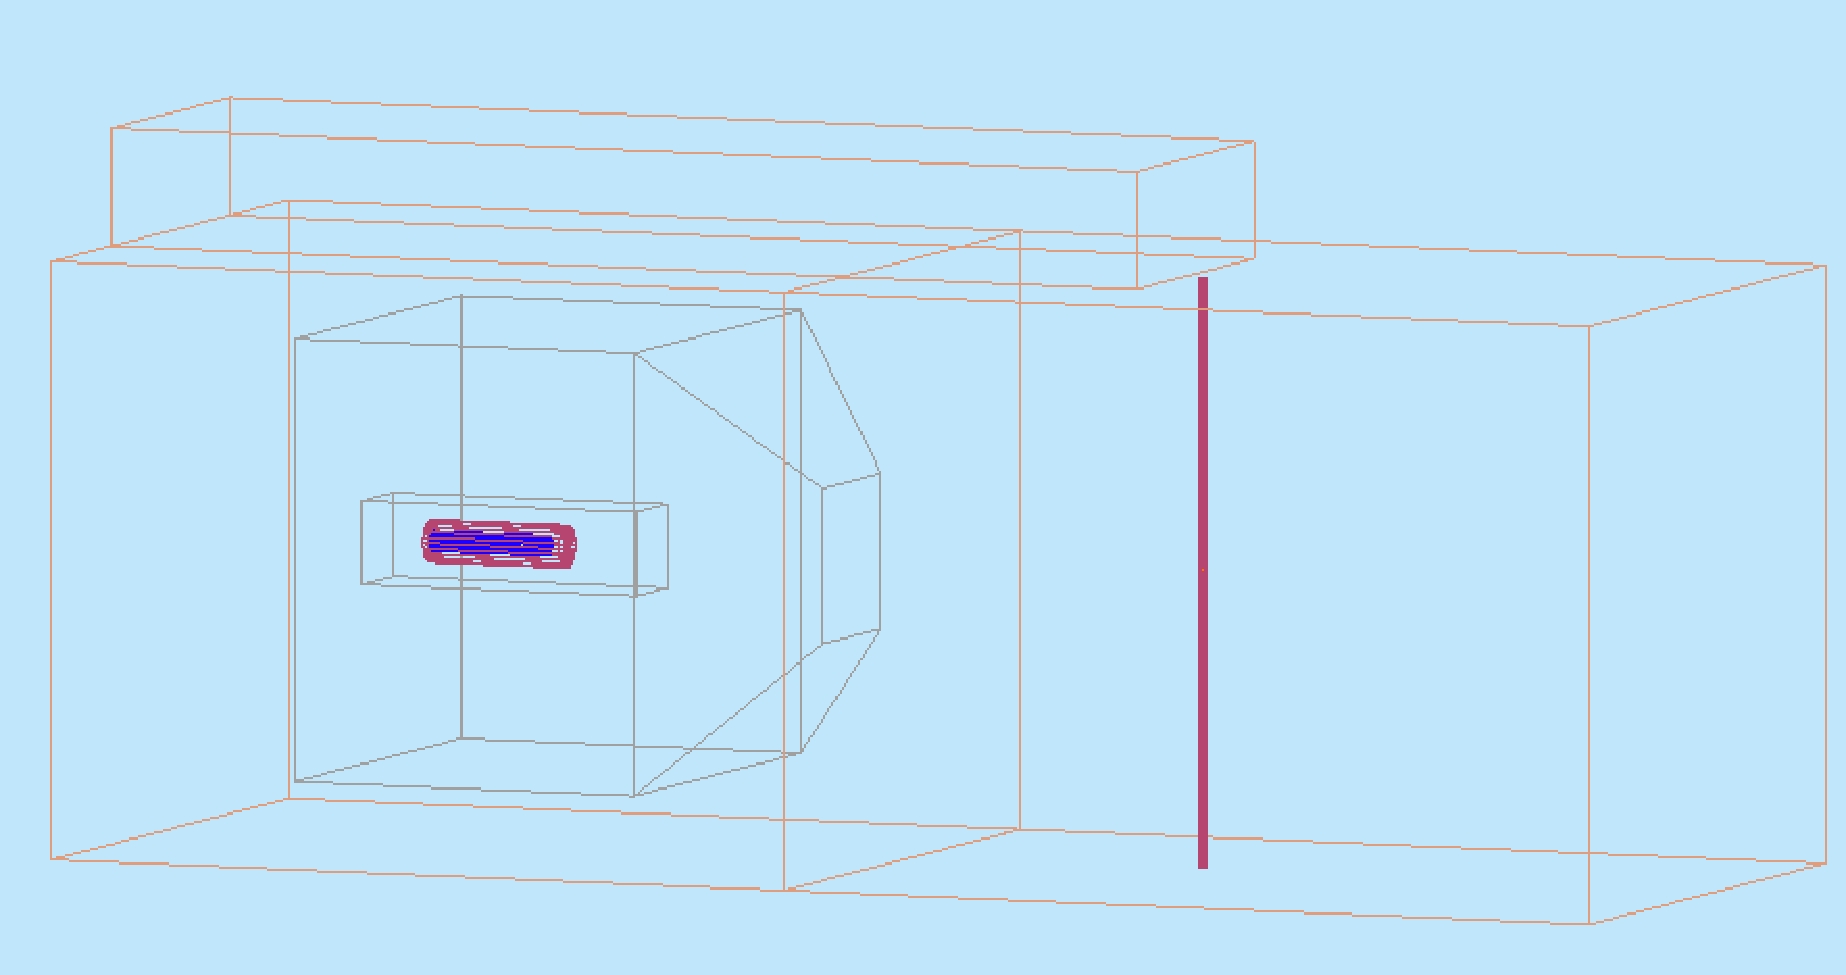
\includegraphics[width=12.5cm]{figs/gemc-bd-dwns.pdf}  
\caption{The geometry/composition  of the beam-dump, the sourraunding concrete bunker and  the soil as implemented in GEMC. The drawings also shows the pipe used to lower the BDX-Hodo detector at the  beam-line depth.}
\label{fig:gemc-bd-dwns}
\end{figure}
\subsection{Muons from beam-dump interaction}
A comparison of muon fluence downstream of the beam-dump (see above for details about the location)
obtained by FLUKA and GEMC are reported in Fig.~\ref{fig:mu-flu-bd}. Considering that low energy muons are absorbed by the bunker-head shielding, to keep the GEMC running time reasonable, only particles with energy grater than 100 MeV ({\tt ENERGY\_CUT=100*MeV}) has been tracked and sampled. A total of 4$\times10^9$ ($9\times 10^6$) EOT have been simulated with GEMC (FLUKA). The comparison of the two simulations shows a perfect agreement in the full energy range where data were generated.
In spite of a factor of $\times$100  less statistics, FLUKA shows, as expected, smaller error bars. This reflects the optimised weight biasing used by the simulation to generate high statistics for the low probability processes keeping the total number of events limited.
To penetrate  the concrete shielding and the soil, a minimum energy of  E$_\mu>4$ GeV is required. With this energy cut,   the integrated number of muon per EOT results in $4.8\pm 0.1 \times 10^{-7}$ ($5.5\pm 0.2 \times 10^{-7}$) for GEMC and FLUKA respectively.
Figure~\ref{fig:mu-flu-bd-2d} shows the correlation between the muon energy and the azimuthal angle (with-respect-to the beam axes): the regions  populated in both simulations show a similar shape.

\begin{figure}[h!] 
\center
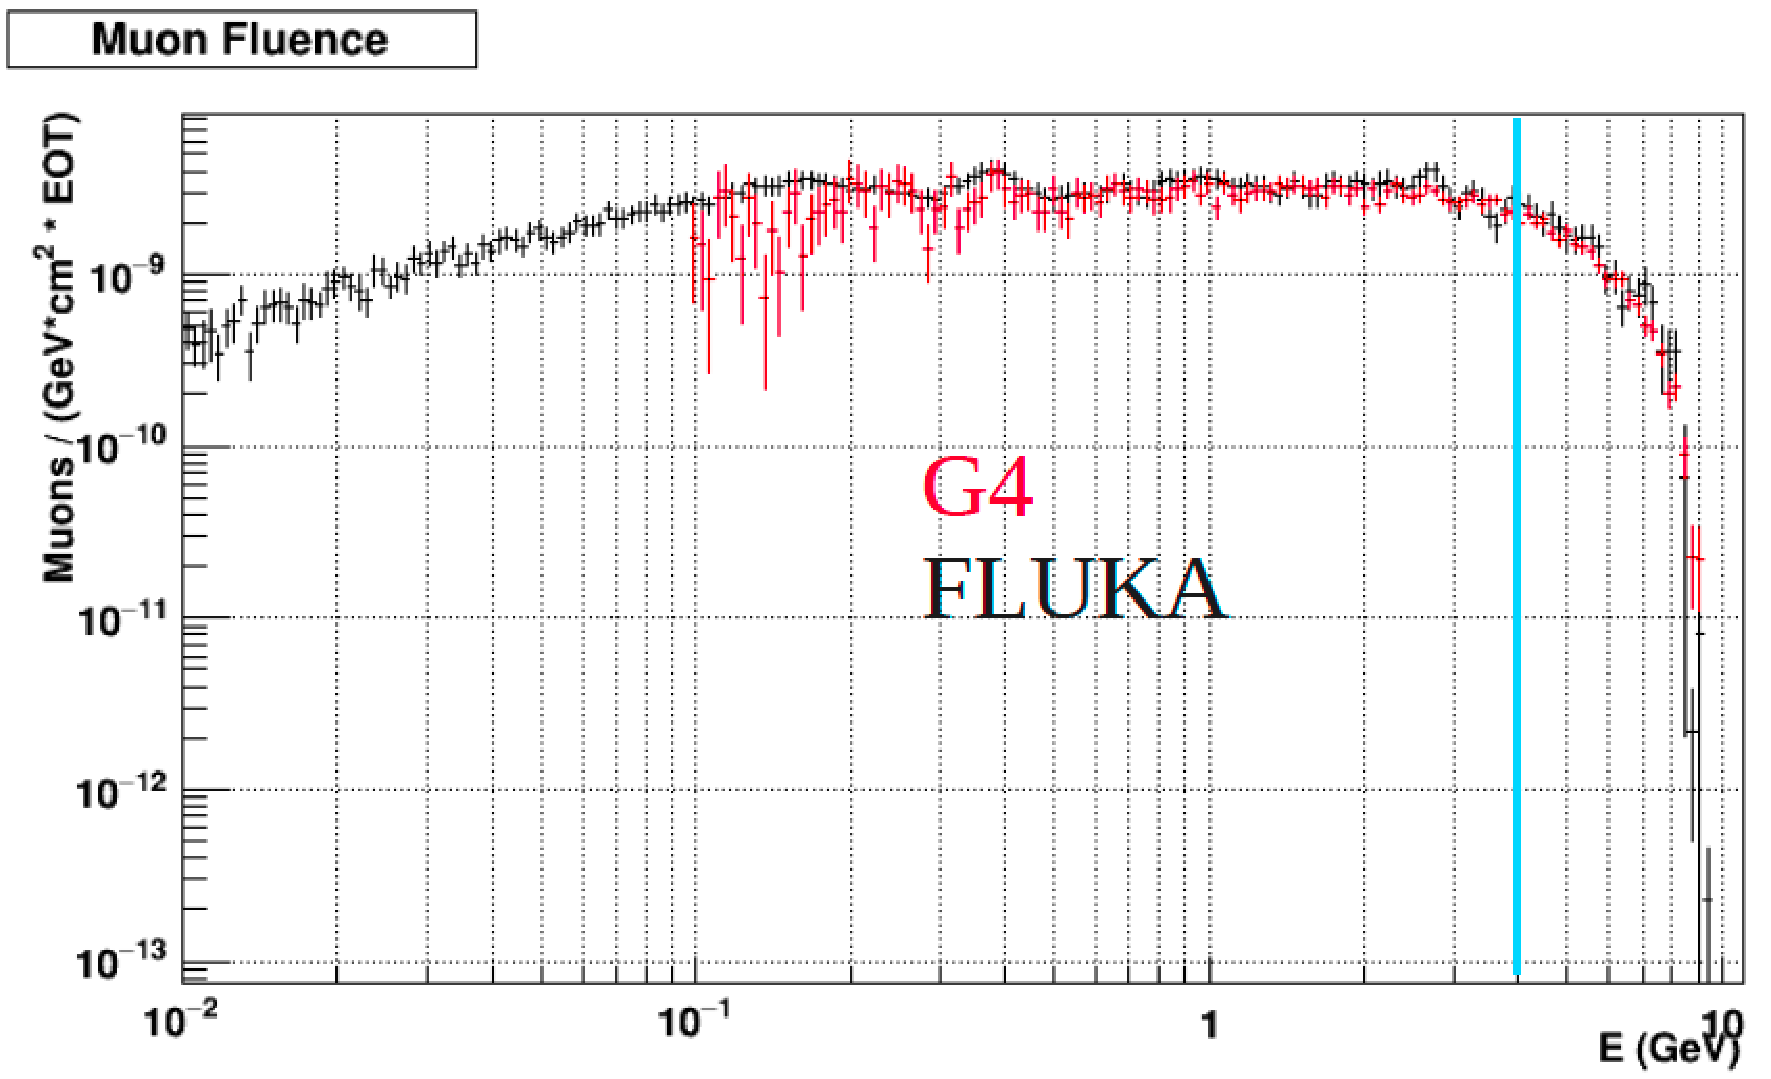
\includegraphics[width=8.5cm]{figs/mu-flu-bd.pdf}
\caption{Muon fluence downstream of the beam-dump obtained by FLUKA (black) and GEMC (red). The GEMC simulations started at E$\mu=$100 MeV.}
\label{fig:mu-flu-bd}
\end{figure}

\begin{figure}[h!] 
\center
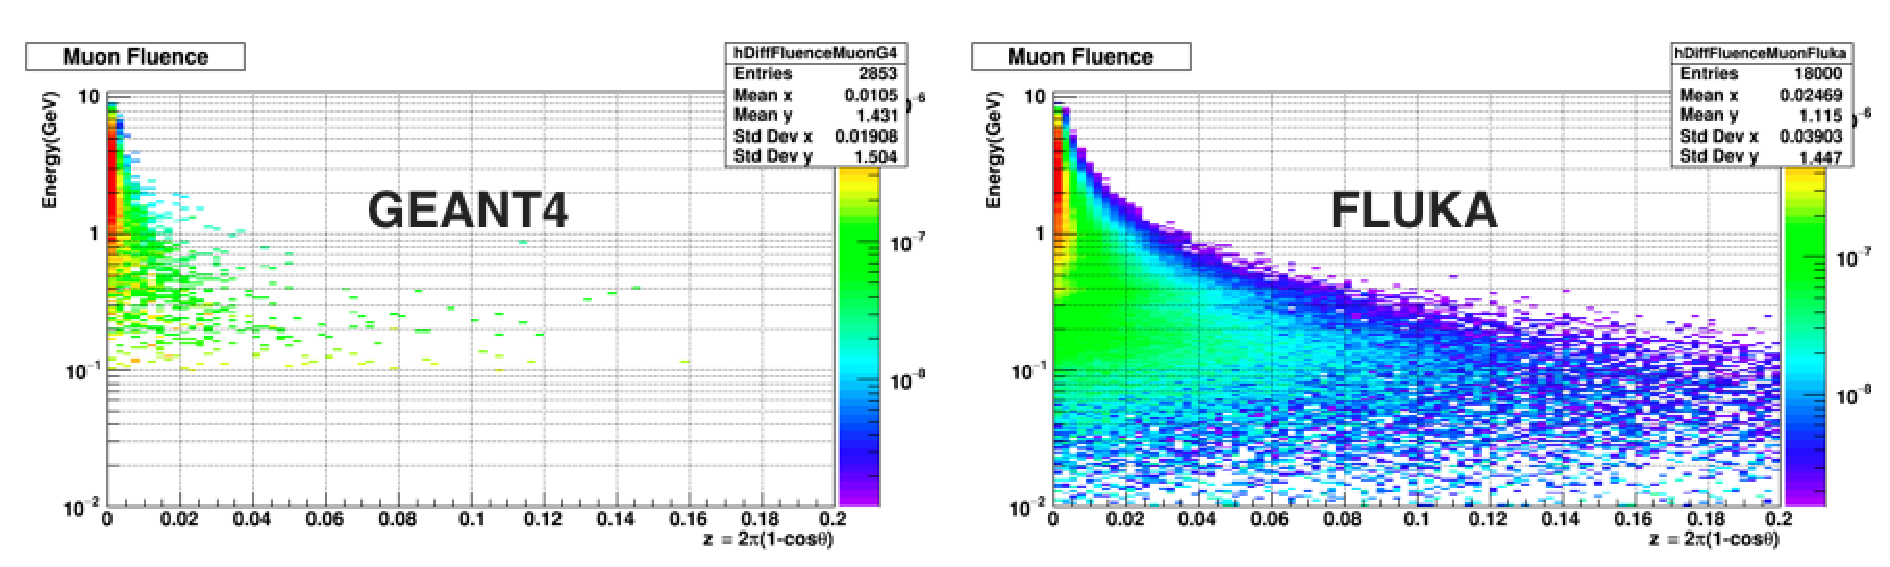
\includegraphics[width=16cm]{figs/mu-flu-bd-2d.pdf} 
\caption{Energy vs. azimuthal angle of muons crossing the flux detector located downstream of the beam-dump obtained by FLUKA  and GEMC.}
\label{fig:mu-flu-bd-2d}
\end{figure}


\subsection{Sampling  and particle transport}\label{sec:sampling}
The good agreement between two independent simulation tools (FLUKA and GEMC)  gives us confidence about reliability of the obtained results. Both methods have pros and cons. FLUKA shows a superior speed in running but a complicated implementation of  variables of interest  (e.g. the final output is given via {\it scores} such as fluence or distribution in specific locations  need to be pre-defined). GEMC (GEANT4) tracks particles in all volumes providing a straightforward  output (particle four-momenta) in the desired flux detector but requires an un-practical running time to collect a reasonable statistics (in particular when an em shower is involved). In the following we describe how we overtook these difficulties.

\subsubsection{Muons - GEMC}\label{sec:gmc-mu}
We used GEMC to simulate muons. To make the  process more efficient, we followed the   procedure described below: 
\begin{itemize}
\item  we used a low statistic sample of EOT to simulate the interaction of the 11 GeV electrons with the beam-dump;
\item  we sampled the muon flux and variables (momentum, azimuthal angle and transverse position)  on a flux detector located downstream of the beam-dump;
\item we used  distributions obtained  in the  previous step as input of a custom event-generator to produce a high statistic muon sample;
\item we used GEMC to transport muons  downstream of the beam-dump all the way down to the desired location(s) of  BDX-Hodo;
\item  we implemented  the  BDX-Hodo response in GEMC to realistically describe the muon detection.
\end{itemize}
The area where  muons are sampled from the primary beam/dump interaction and used  as source in the custom-made event generator is shown in Fig.~\ref{fig:mu-gen}.

\begin{figure}[h!] 
\center
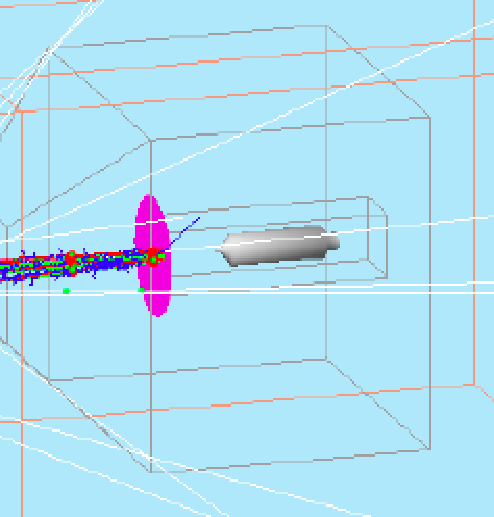
\includegraphics[width=12cm]{figs/mu-gen.pdf}   
\caption{The  $\mu$ sampling/generation area is the surface surrounded by  the magenta circle.}
\label{fig:mu-gen}
\end{figure}


Figure~\ref{fig:mu-sampling} shows the muon distributions (energy vs azimuthal angle and radial distance from the beam line) downstream of the beam-dump, as obtained by the full GEMC simulation of  11 GeV electrons hitting the beam-dump.
The left panel of Fig.~\ref{fig:mu-sampling-extract} shows the  distributions obtained by running the full simulation with GEMC compared to  the custom event generator results. 
As a check, the right panel of the same figure  shows the  comparison in the location of interest ($\sim 20$ m downstream of the beam-dump).
The difference in the error bar size indicates the improvement obtained by adopting this procedure.
\begin{figure}[h!] 
\center
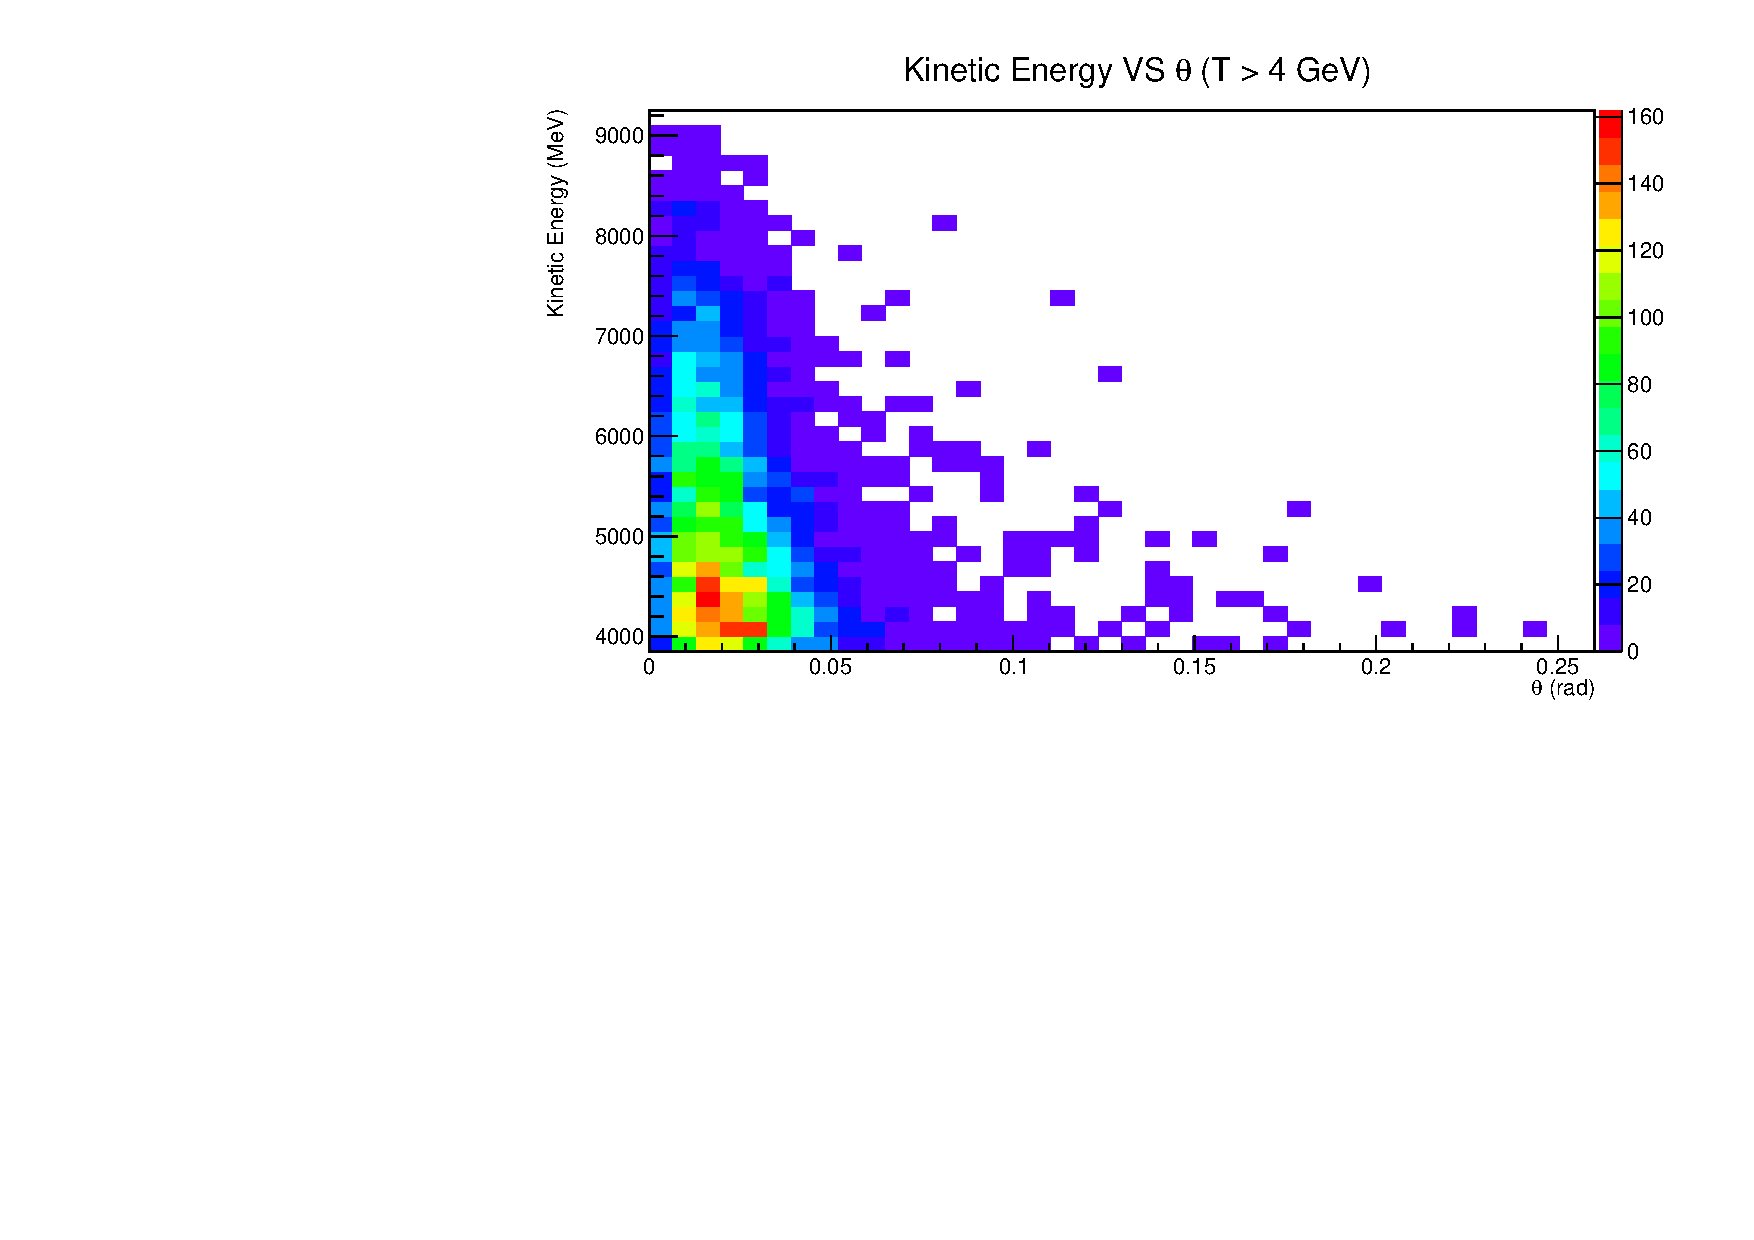
\includegraphics[width=7.5cm]{figs/EkinVStheta.pdf}
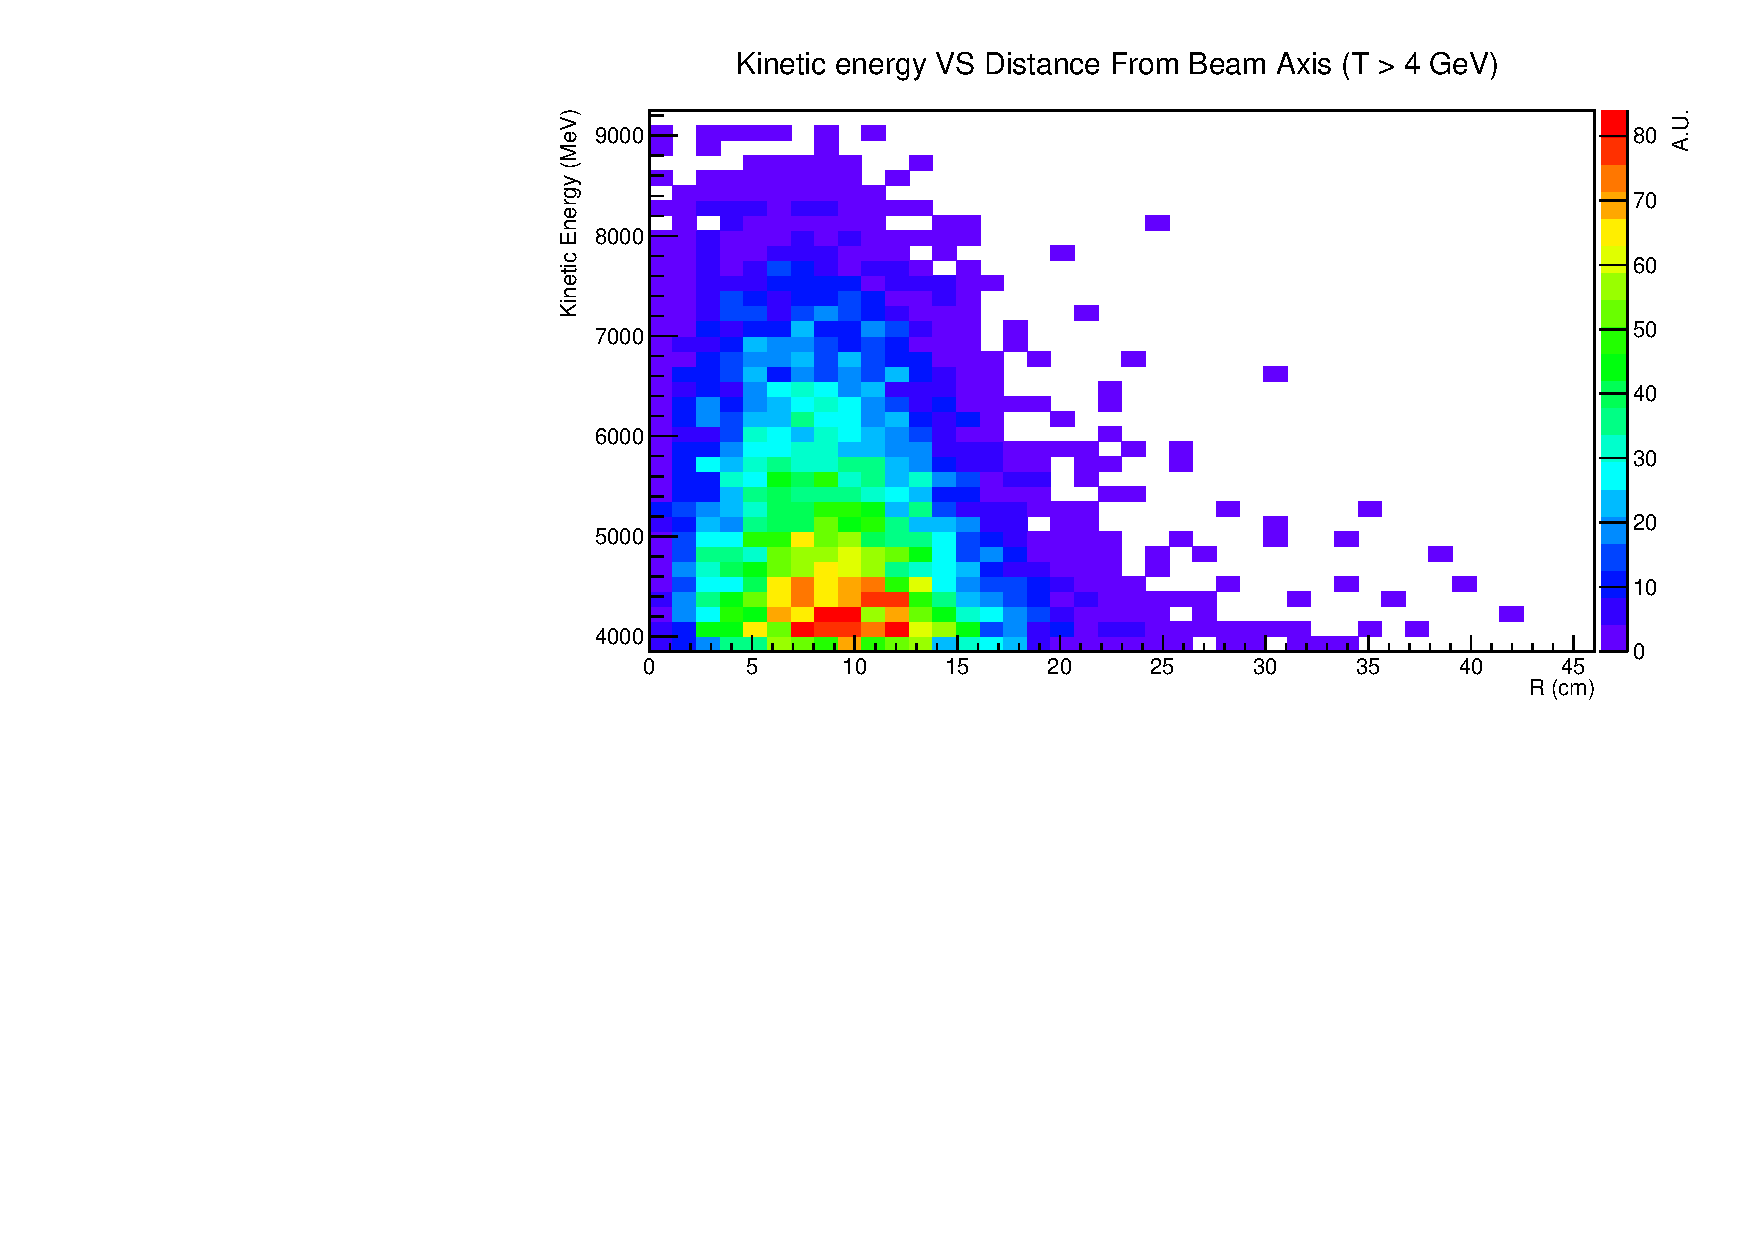
\includegraphics[width=7.5cm]{figs/EkinVSR.pdf}
\caption{Muon kinetic energy vs. azimuthal angle (left) and distance (right) from the beam-line axes as obtained by the full GEMC simulation.}
\label{fig:mu-sampling}
\end{figure}
\begin{figure}[h!] 
\center
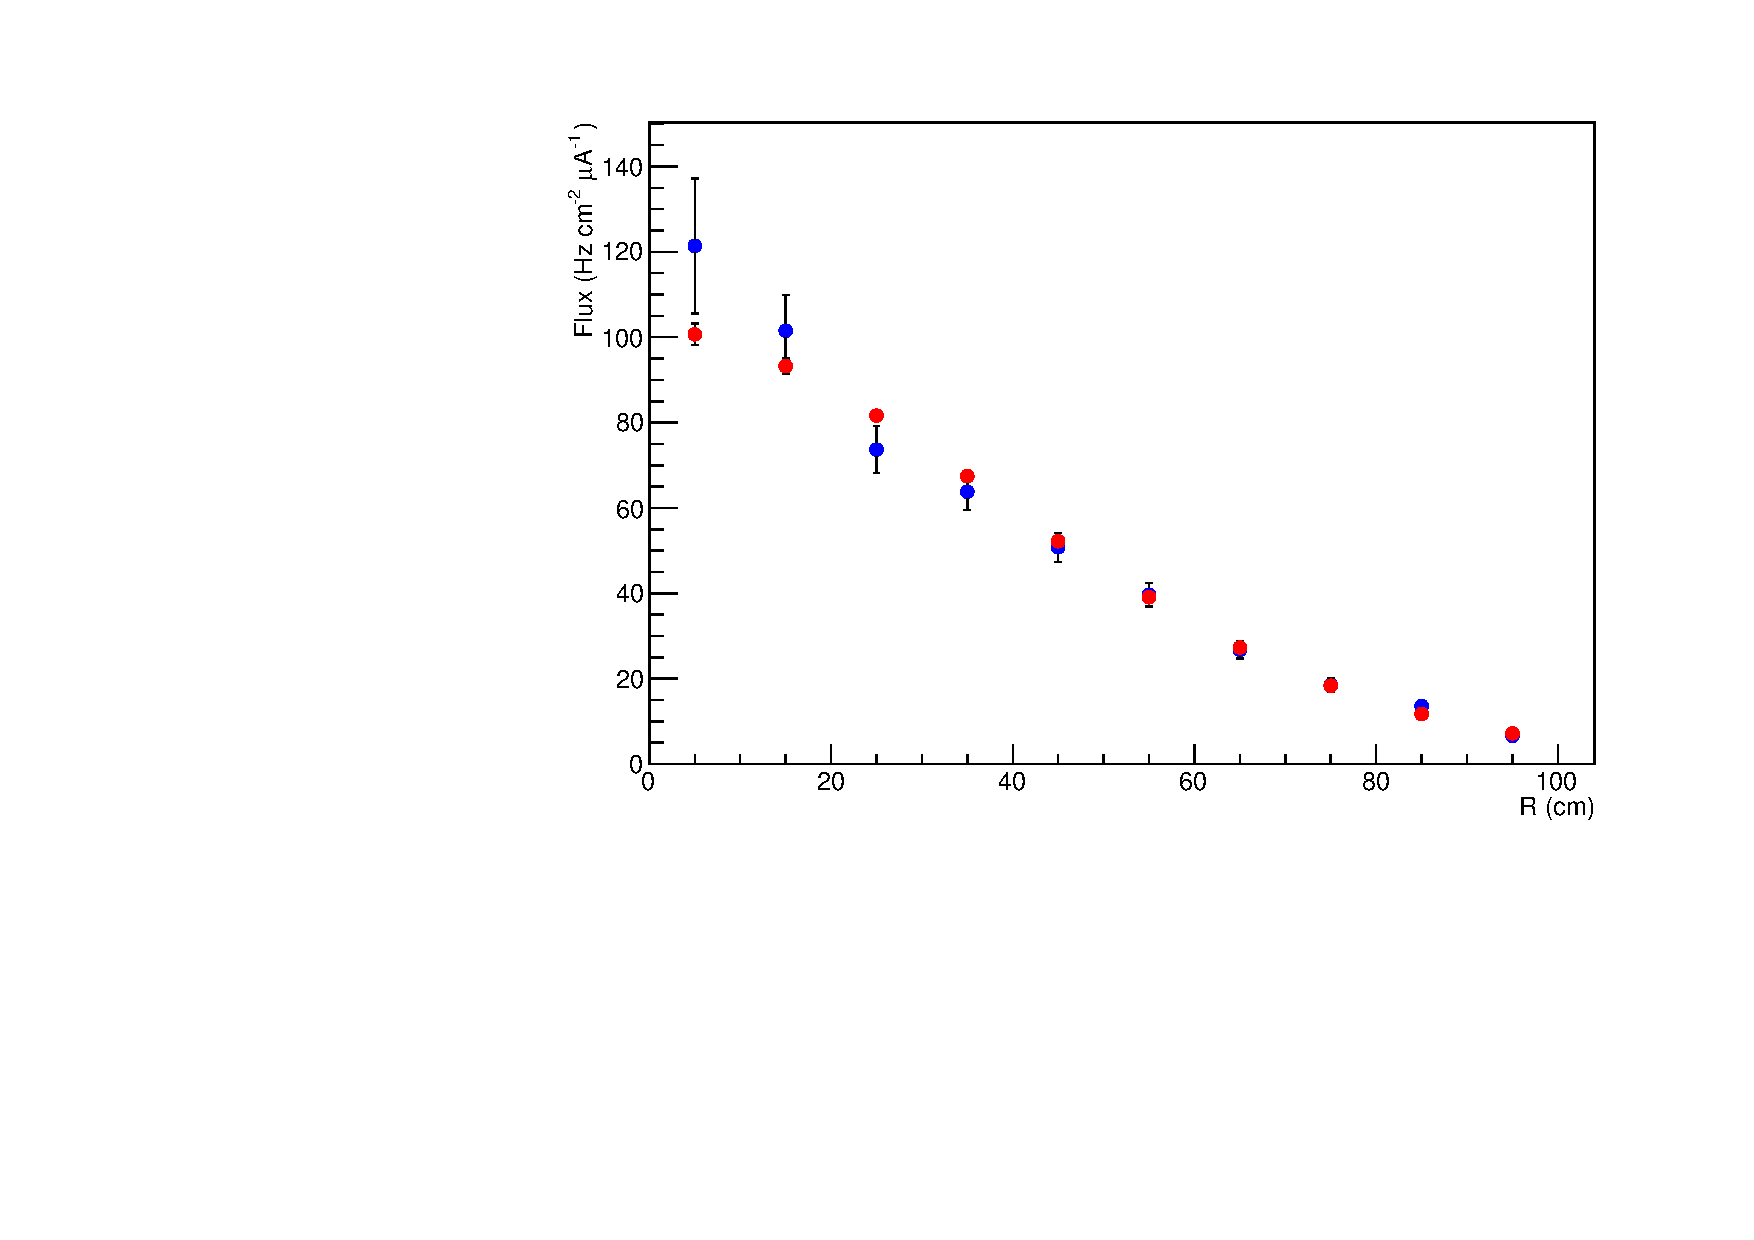
\includegraphics[width=7.7cm]{figs/SimVSGen.pdf}
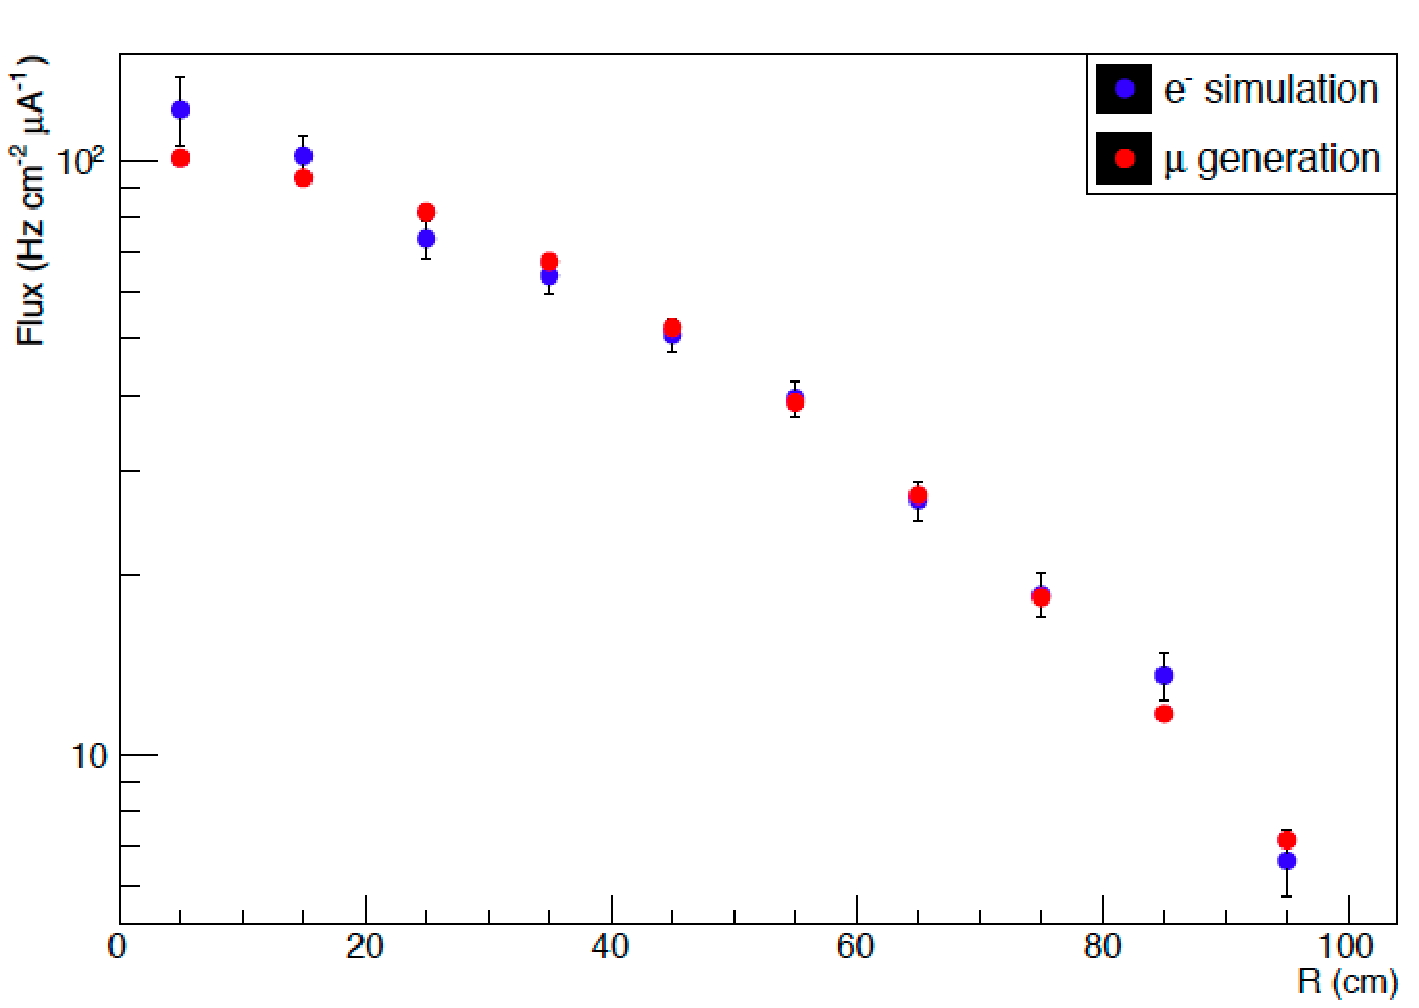
\includegraphics[width=7.0cm]{figs/mu-comp-far.pdf}
\caption{Muon flux as a function of the radial  distance from the beam axes obtained by GEMC (blue) and by the custom event-generator (red) at the sampling/generation location (left) and in the region of interest (right), $\sim 20$ m downstream of the beam-dump.}
\label{fig:mu-sampling-extract} 
\end{figure}


\begin{figure}[h!] 
\center
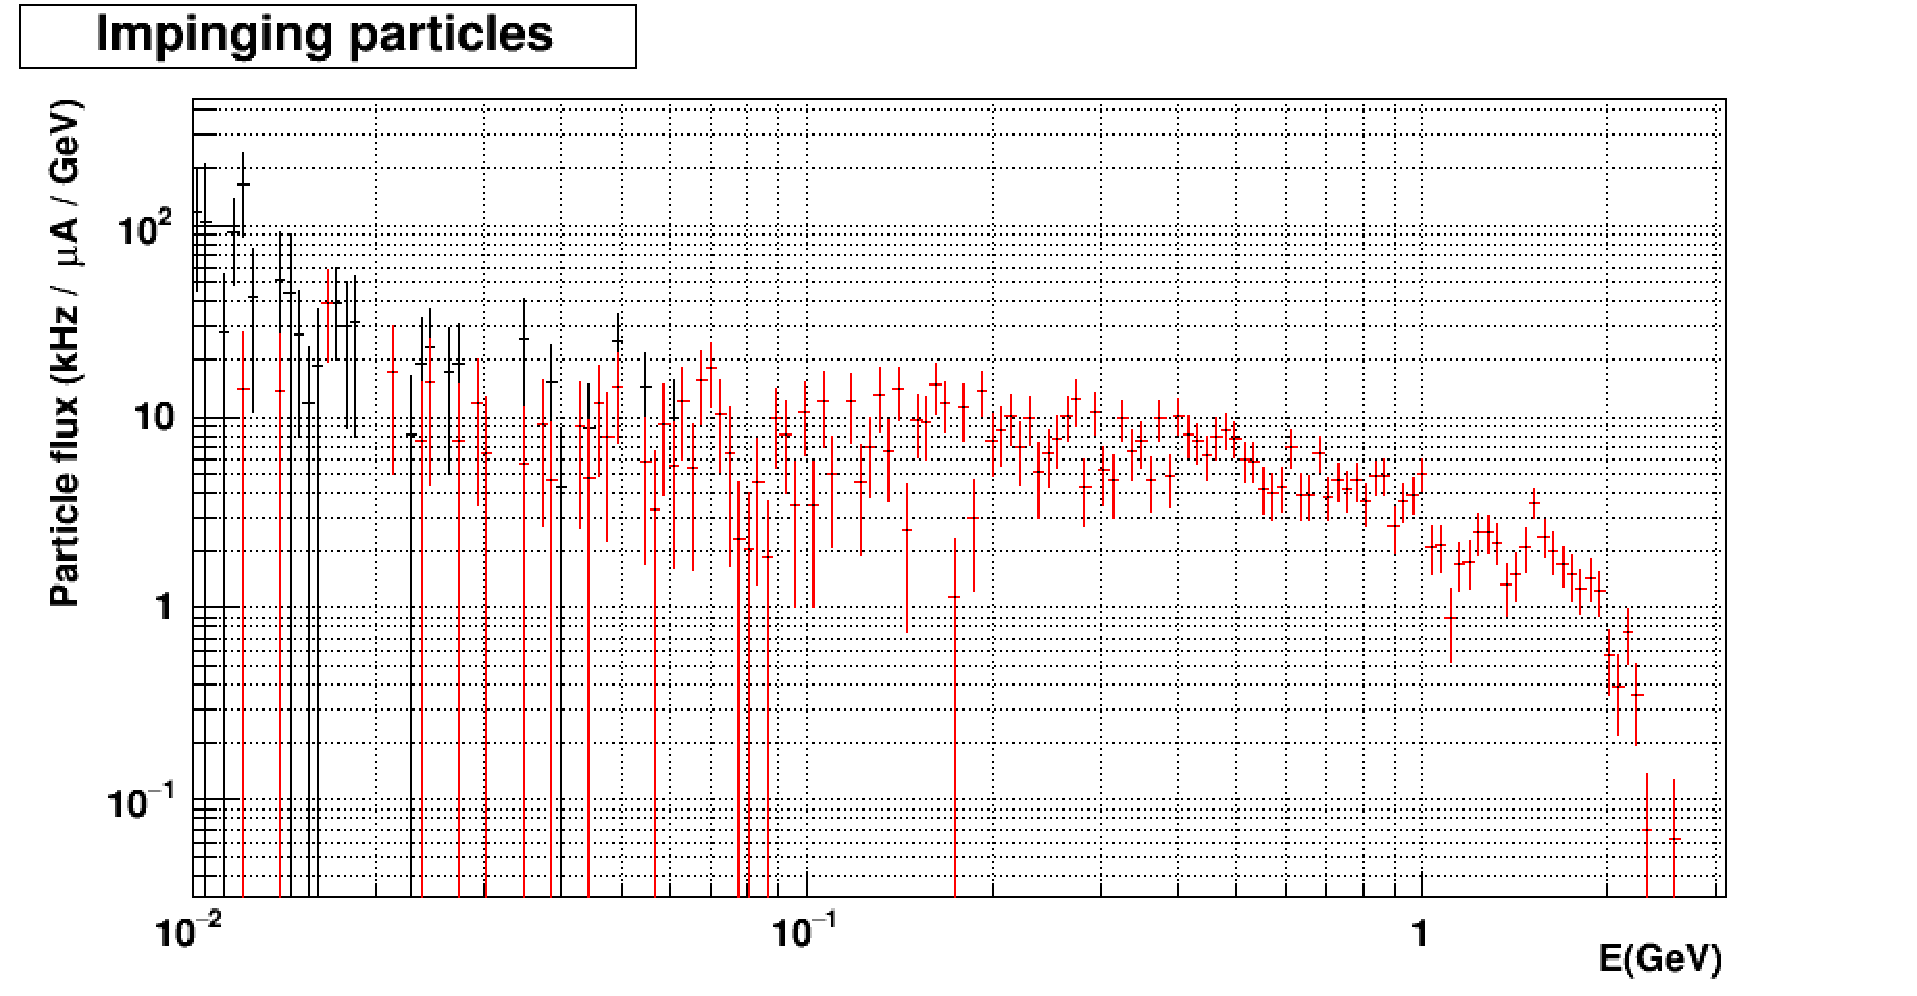
\includegraphics[width=15cm]{figs/fig10.pdf}    
\caption{Fluence  on  CsI(Tl) crystal of  all crossing particles (black) and muons only (red). The crystal is located in the region of interest $\sim 20$ m downstream of the beam-dump. }
\label{fig:bg-csi}
\end{figure}

\subsubsection{Background - FLUKA} 
We used FLUKA to estimate the background expected in the BDX-Hodo detector.
We simulated an 11 GeV electron-beam interacting with the beam-dump, propagate all particles to the location of interest obtaining the fluence on the CsI(Tl) surface.
Figure ~\ref{fig:bg-csi} shows the resulting fluence per EOT as a function of energy  for all particles (black) and muons only (red).
As expected,  muons are the only high energetic  particles reaching  the crystal while other species (neutrons mainly) account for the low energy of the spectrum. More details are reported in Sec.~\ref{sec:results}.
\begin{figure}[h!] 
\center
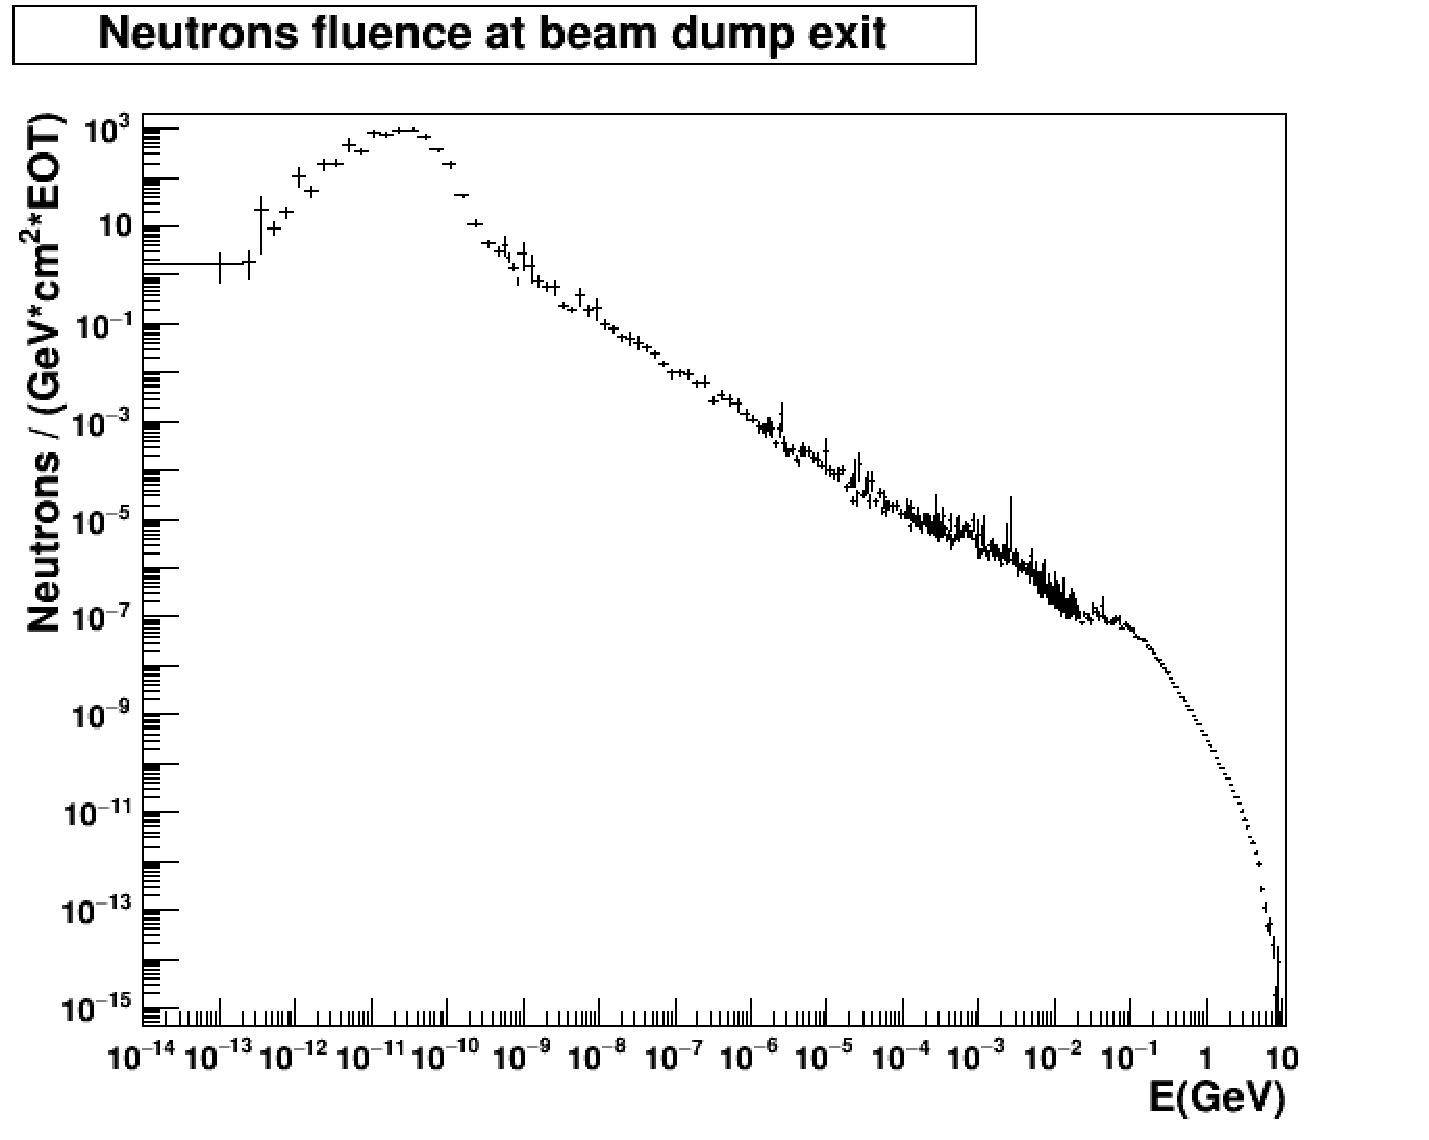
\includegraphics[width=7.5cm]{figs/NeutronsDump_1D.pdf}    
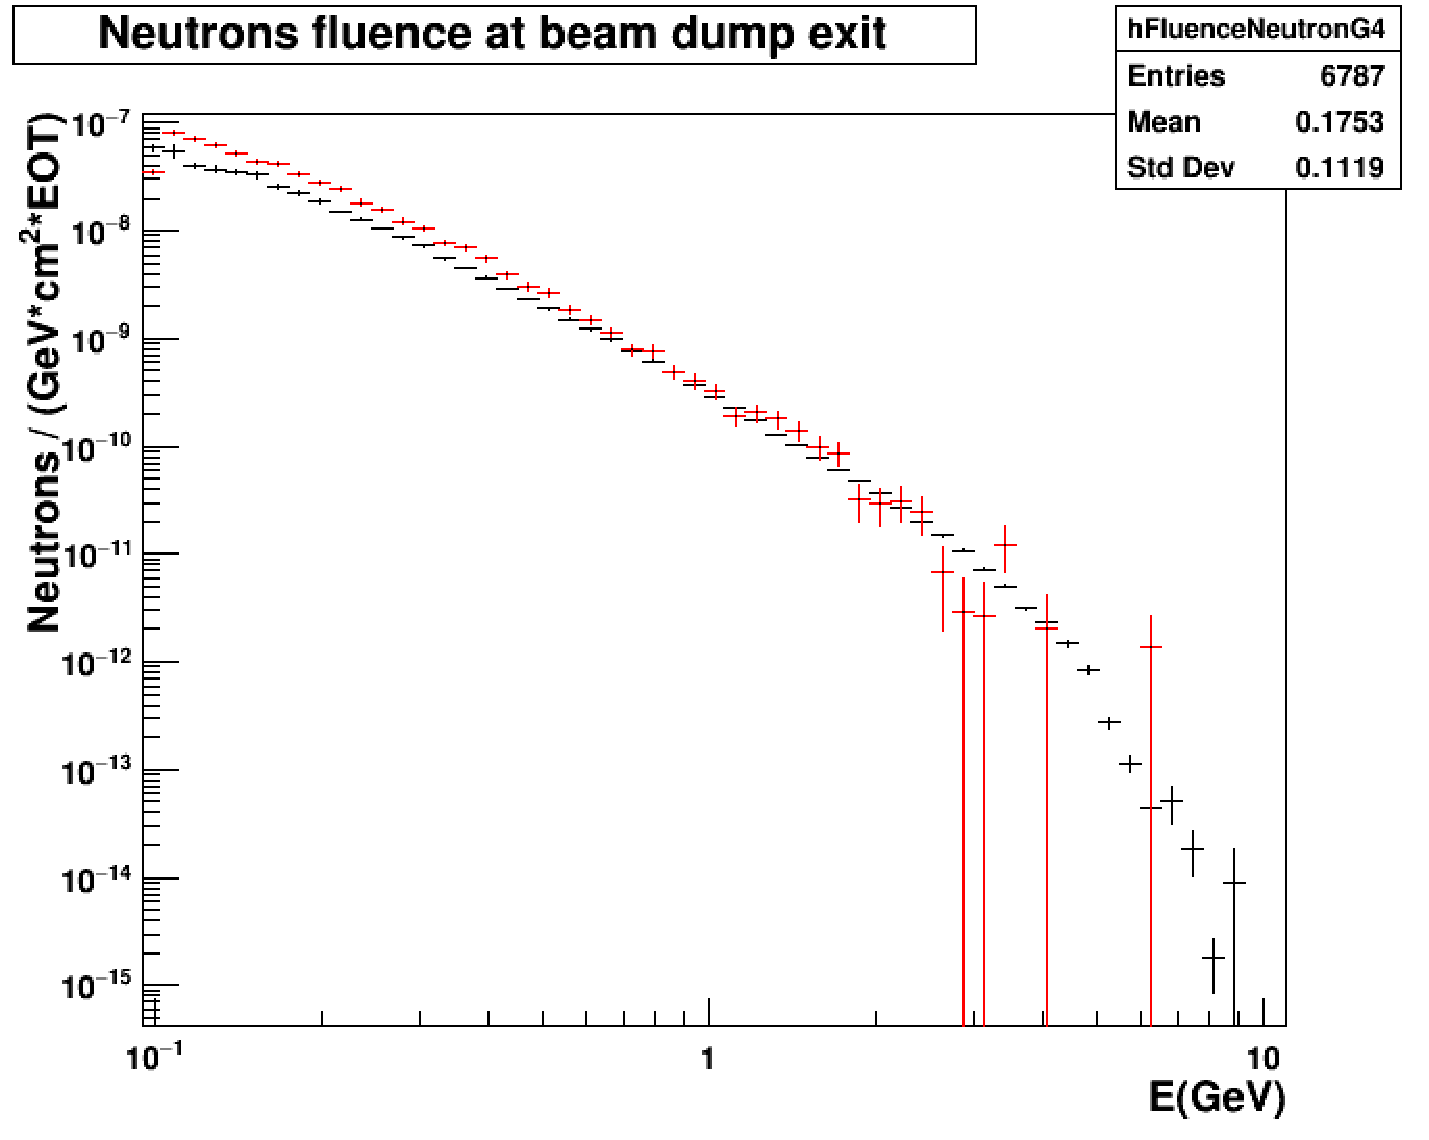
\includegraphics[width=7.5cm]{figs/NeutronsDumpComparison_1D.pdf}   
\caption{Neutron spectrum downstream of the the dump obtained by full FLUKA simulation (left). The right panel shows  the comparison between FLUKA (black) and GEMC (red) for the high energy part pf the spectrum.}
\label{fig:n-comp}
\end{figure}

It's interesting to note that the spectrum of  high energy neutrons , T$_n>$ 100 MeV,  (sampled downstream of the dump)  obtained by GEMC is in good agreement with FLUKA (see Fig.~\ref{fig:n-comp}). The agreement indicates  that, in this energy range, both simulation tools are reliable. 

Another interesting aspect of the neutron spectrum is shown in Fig.~\ref{fig:n-lowE}. The energy spectrum (sampled downstream of the dump) obtained by FLUKA by RadCon (Ref.~\cite{jnote-bd}) is compared to the same plot obtained by our FLUKA simulations. The two models differ in the implementation of the  beam-dump vault: a detailed description of the material surrounding the dump,  that includes air and concrete,  versus a simplified geometry/material description.   The effect is clearly visible in the low energy part of the spectrum (while the high energy part is almost identical) proving that a detailed description of the dump enclosure is necessary to correctly describe the low energy backgrounds.
\begin{figure}[h!] 
\center
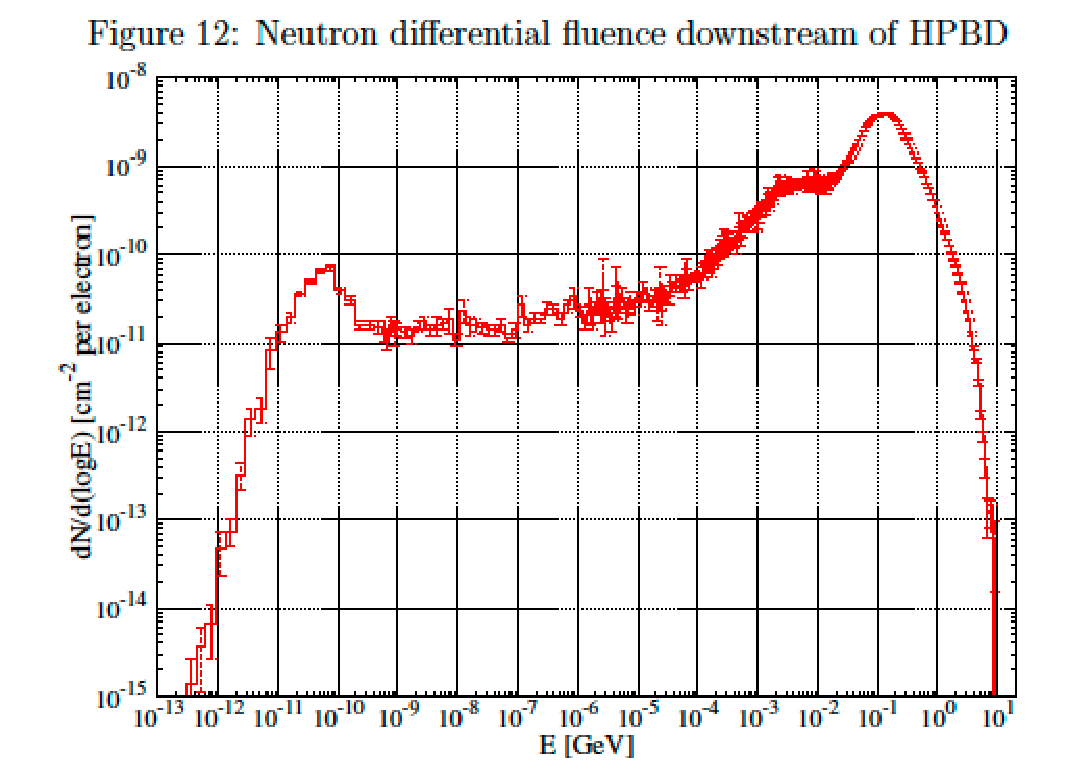
\includegraphics[width=7.5cm]{figs/bg-lowN-george.pdf}    
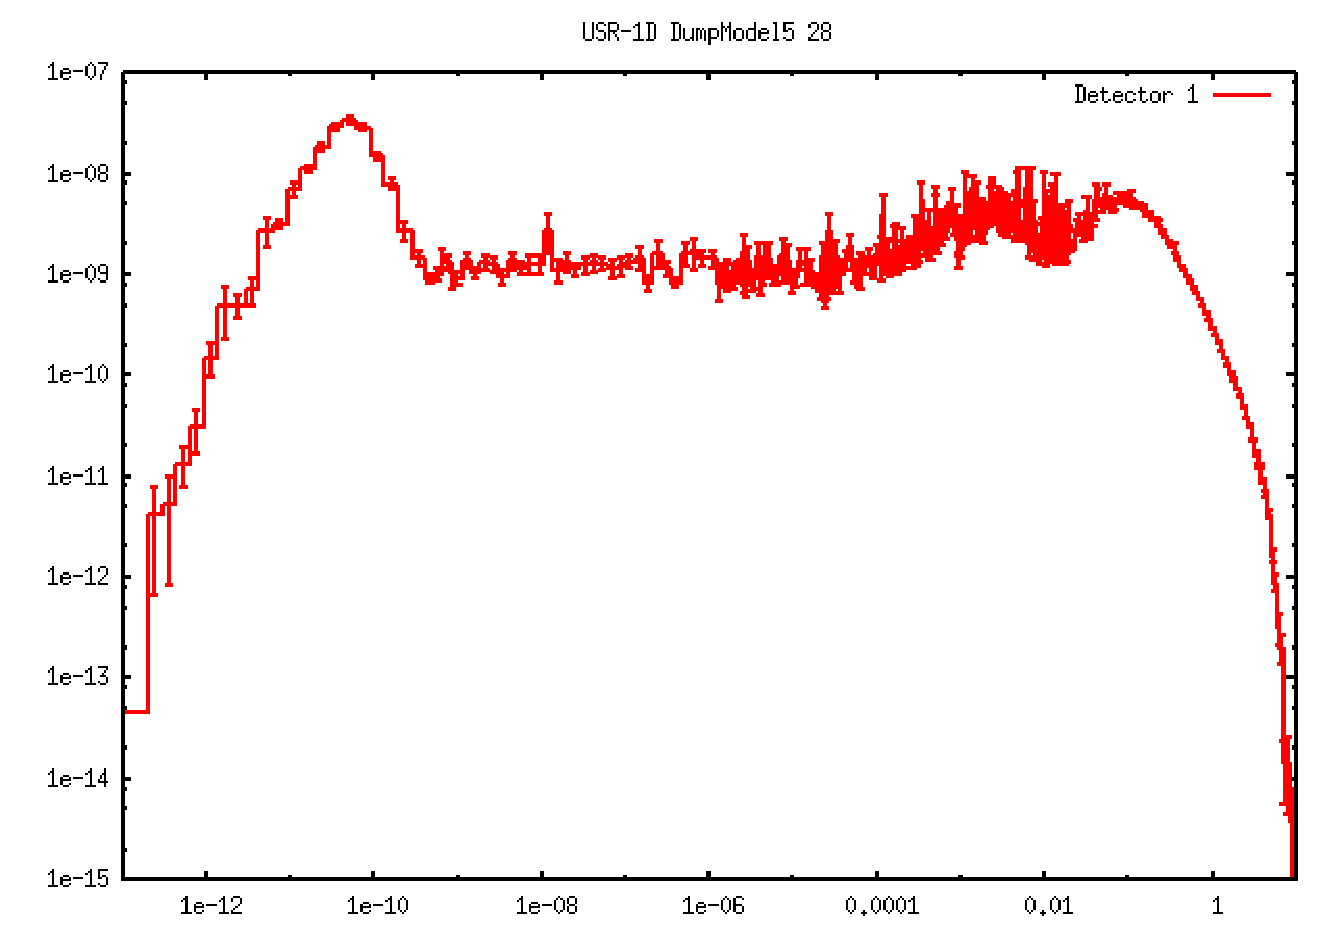
\includegraphics[width=7.5cm]{figs/NeutronsDumpComparisonDnDlogE_1D.pdf}   
\caption{Comparison of neutron energy spectrum obtained by FLUKA, sampled downstream of the beam-dump with a simplified geometry (left) and including vault sourrounding materials (right). The numeber of low energy neutrons significantly increases when the reflection on the wall is considered.}
\label{fig:n-lowE}
\end{figure}
\\ \\ 
Muon and background flux  at  the location of interest will be discussed in details in the Sec.~\ref{sec:results} after presenting the BDX-Hodo detector in the next Section. 




\clearpage
\section{Test set-up}
\label{sec:setup}
\begin{figure}[h!] 
\center  
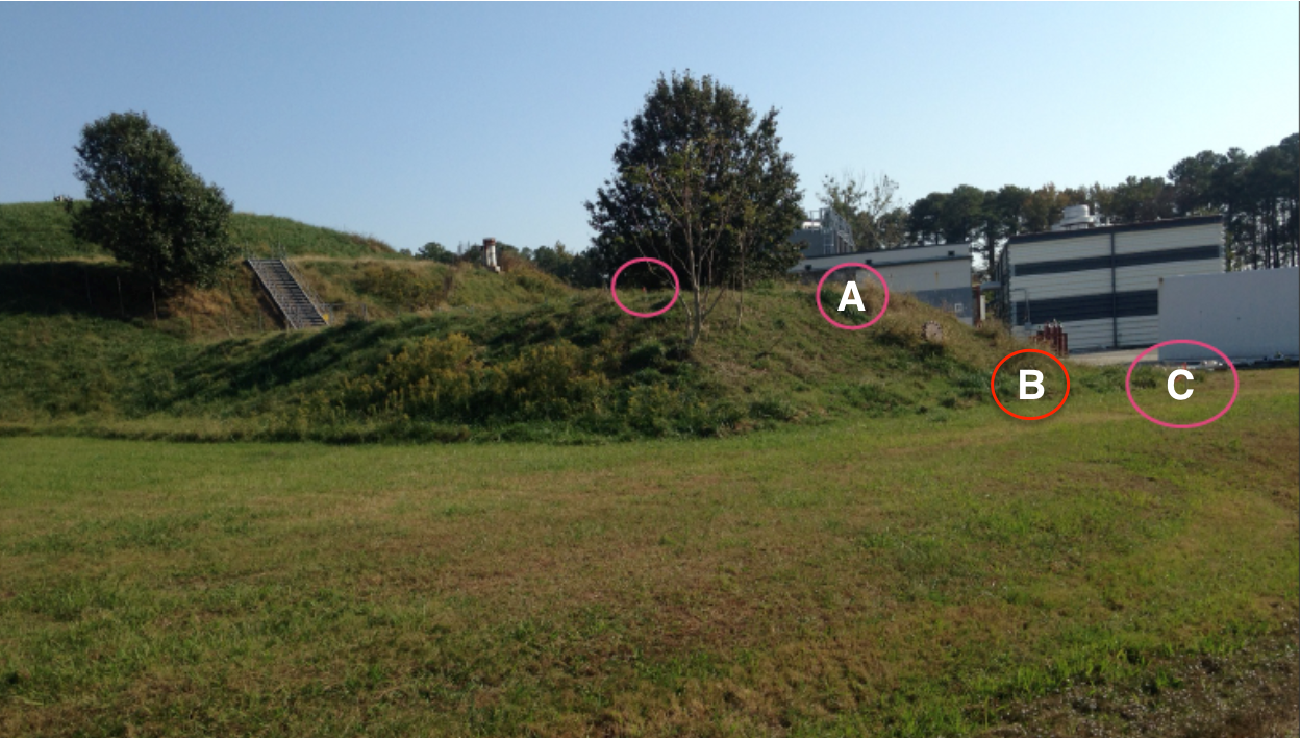
\includegraphics[width=11.5cm]{figs/ds-area.pdf}   
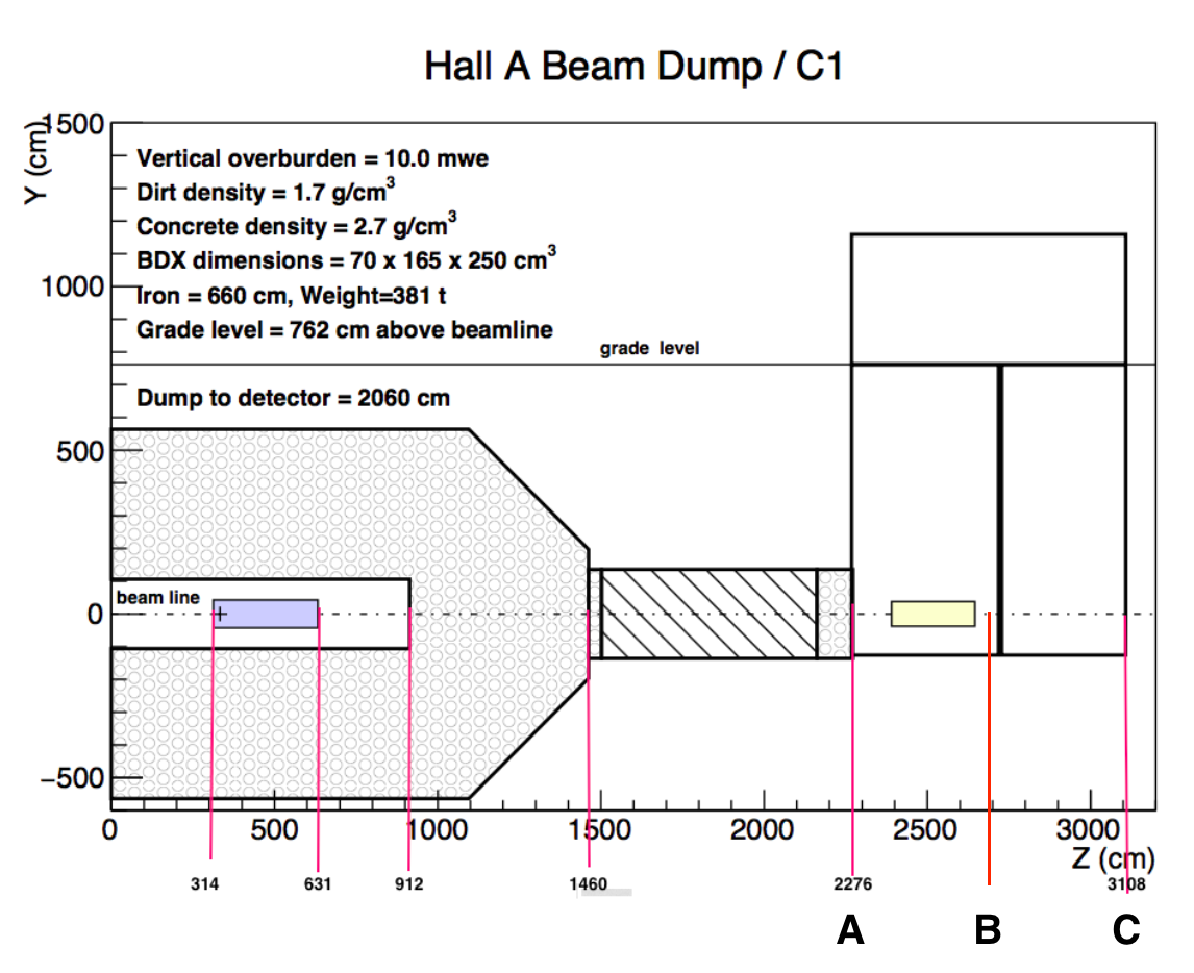
\includegraphics[width=11.5cm]{figs/test-plan.pdf}  
\caption{The area downstream of the Hall-A beam-dump and the studied test locations.}
\label{fig:ds-area}
\end{figure}

\subsection{Detector location}
The area downstream of Hall-A beam-dump is shown in Fig.~\ref{pic:ds-area}  together with the corresponding location with-respect-to  
the new  underground facility proposed in PR-16-001~\cite{bdx-proposal}. The three positions, indicated with markers {\bf A, B}  and {\bf C},  correspond to the hall entrance (22.4 m downstream of the beam-dump entrance), a point in the middle  (25.2 m) and the exit (28 m), respectively. The experimental set-up we are proposing  assumes to dig a well and insert a pipe in one (or more) of these locations. The BDX-Hodo detector will be lowered in the pipe and muon flux sampled at different height wrt. the beam-line nominal height. The muon flux profiles in Y (vertical direction), measured in  different location in Z (distance from the dump) will allow us to compare the absolute and relative MC predictions. 

\subsection{The BDX-Hodo detector}
The detector used to measure the muon and neutron radiation in the proximity of the new BDX underground facility will  make use of a BDX ECal CsI(Tl) crystal sandwiched between a set of segmented plastic scintillators.
A CAD representation as well as   cuts with sizes are shown in Fig.~\ref{pic:det-cad}.
\begin{figure}[h!] 
\center
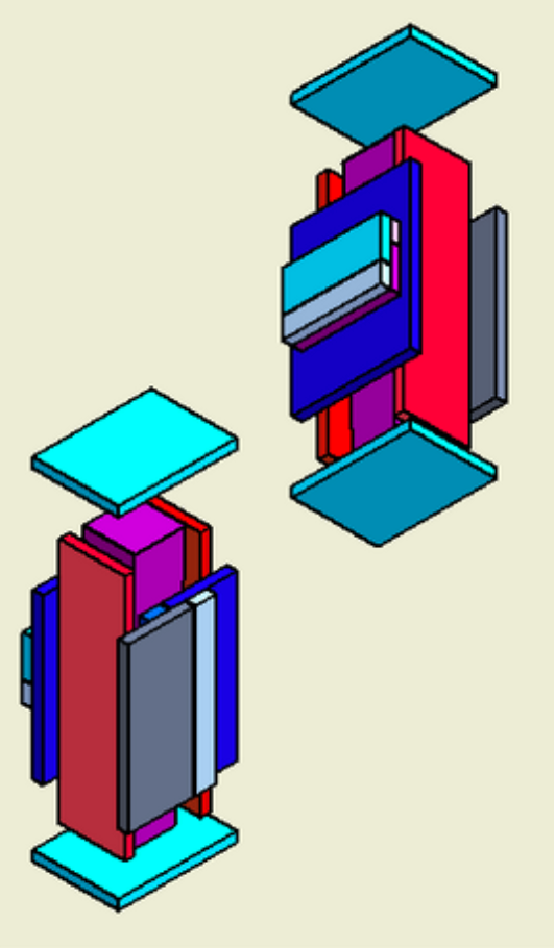
\includegraphics[width=2.9cm]{figs/det-3d1.pdf}  
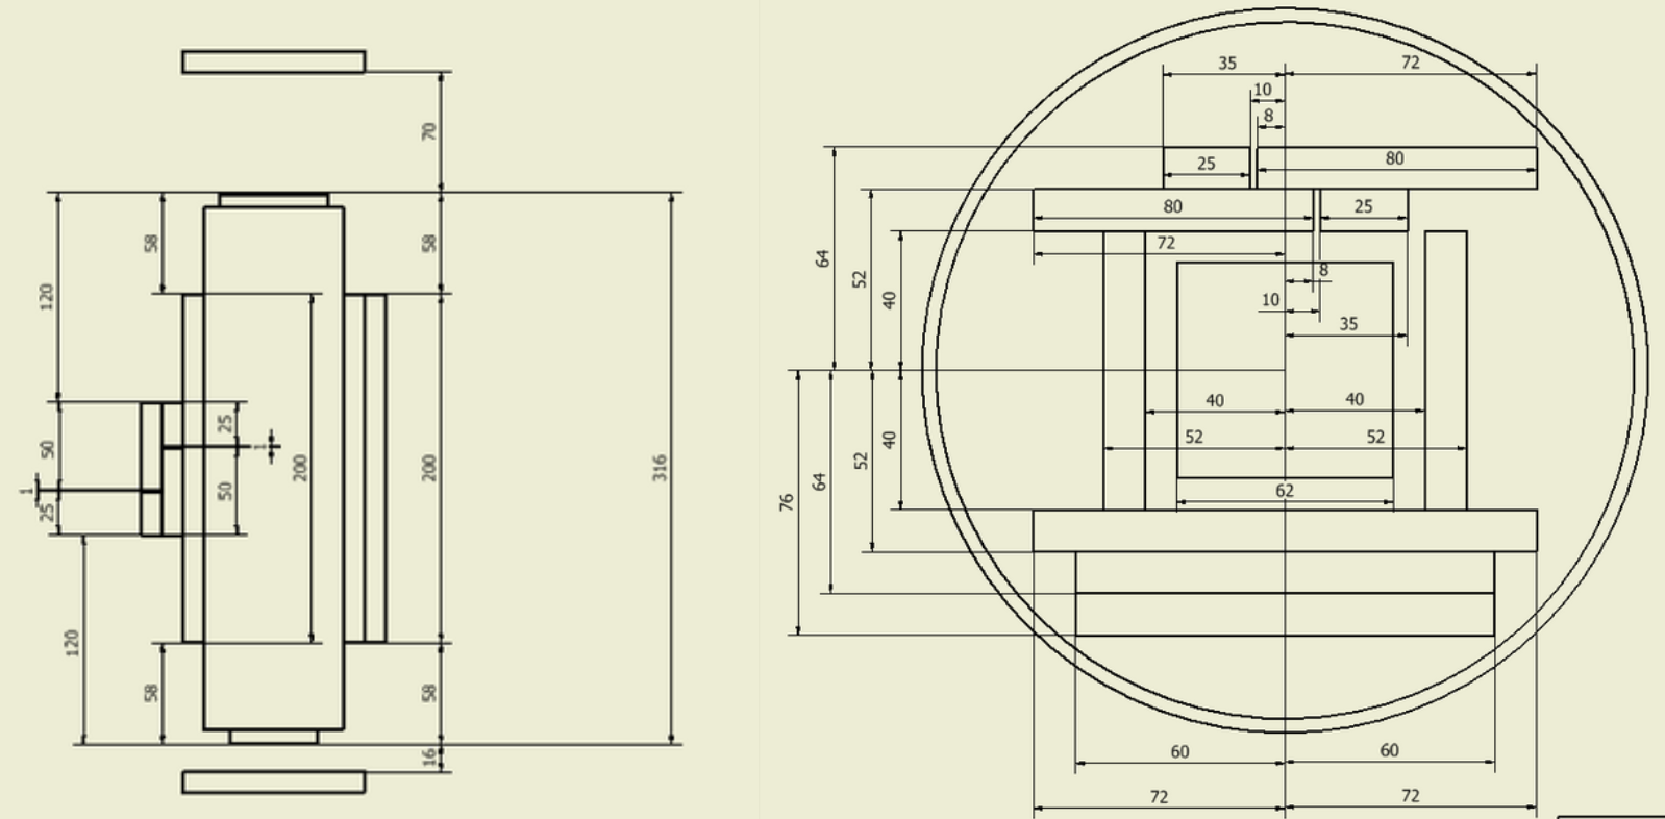
\includegraphics[width=10.1cm]{figs/det-3d2.pdf}   
\caption{The CAD representation of the BDX-Hodo detector and some drawings with geometry and sizes.}
\label{fig:det-cad}
\end{figure}
The front of the crystal will be equipped with two  layers of plastic scintillators, each of them composed by  a large and a small 1cm-thick scintillators strips. The overlap of the four paddles (each 20 cm long in Y)  results in three independent  2.5 cm channels along the X (horizontal) direction.
The same concept was applied to the  back side of the crystal but with paddles tilted by 90 degrees to define three 2.5 cm independent channels along the Y (vertical) direction. The requirement of a hit in both front and back paddles defines a 3x3 matrix of 2.5x2.5 cm$^2$ pixels providing a cm-like XY position resolution. 
The addition of a larger paddle (20 x 14.4 cm$^2$) on the back provides an enhanced sensitivity   in the unlikely  case rates will be much lower than what estimated by MC simulations.
Four more  paddles covering  the left/right sides and the top/bottom of the crystal will be used to veto cosmic rays and other radiation not associated to the beam direction.
The crystals will be coupled, on the large side,  to a 6x6 mm$^2$ Hamamatsu S13360-6025 SiPM as described in Sec. 3.2.1 of  PR-16-001~\cite{bdx-proposal}. The scintillator paddles will be  made with extruded plastic, each  read out via a WLS fiber coupled to a 3x3 mm$^2$ Hamamatsu S12572-100 SiPM sharing the same technology used in the BDX Inner Veto detector (described in details in Sec. 3.2.2 of  PR-16-001).
Muons produced by the electron beam will be detected by requiring a 5-fold coincidence (two front paddles + CsI(Tl) crystal + two back  paddles).
The detector will be contained  in a 20-cm diameter stainless-steel cylindrical vessel, covered on top and on the bottom by steel lids. The whole assembly will  be water-tight to prevent any water leak inside the vessel. A stainless-steel  extension to the top cover will be used  to run signal and power cables from the detector to the ground.The extension, made by a 1-inch stainless steel pipe,  rigidly attached, will be used also  to remotely control the cylinder rotation and provide a good accuracy in the define the angle wrt. the beam direction.
The electronics necessary to record the 13 (scintillators) + 1 (crystal) channels require 1 fADC board inserted in a VME crate. The full DAQ system (crate + pc)  will be host in a van parked close to the well entrance. The power will be provided by a diesel power generator to minimize the requirements of long extension cords.

\begin{figure}[h!] 
\center
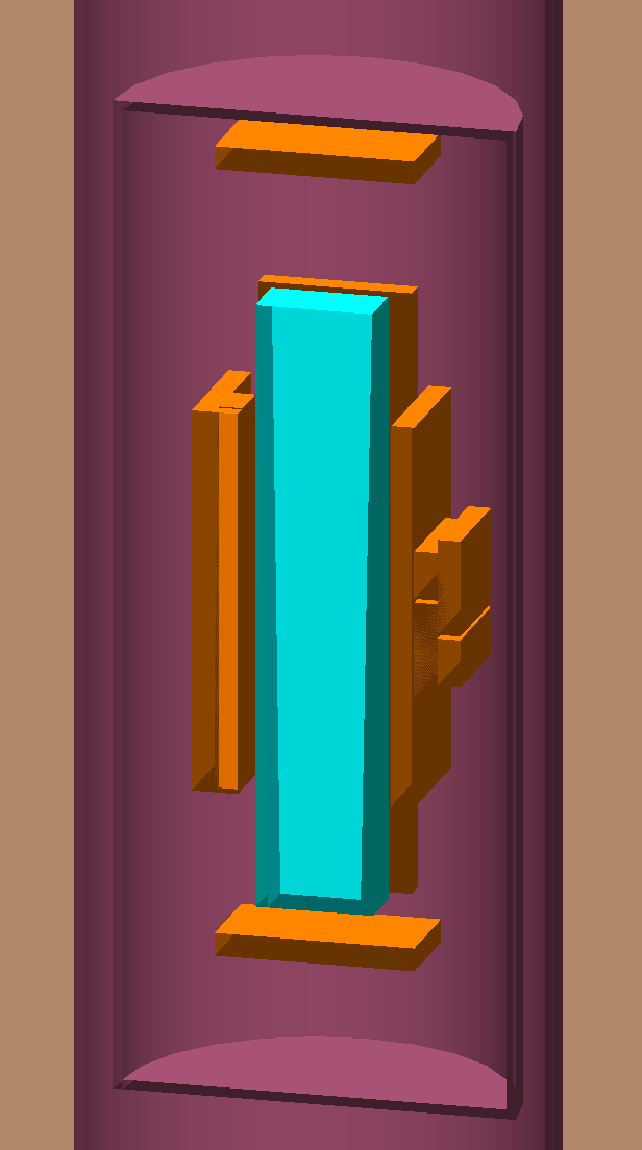
\includegraphics[width=2.99cm]{figs/gemc-3d.pdf}  
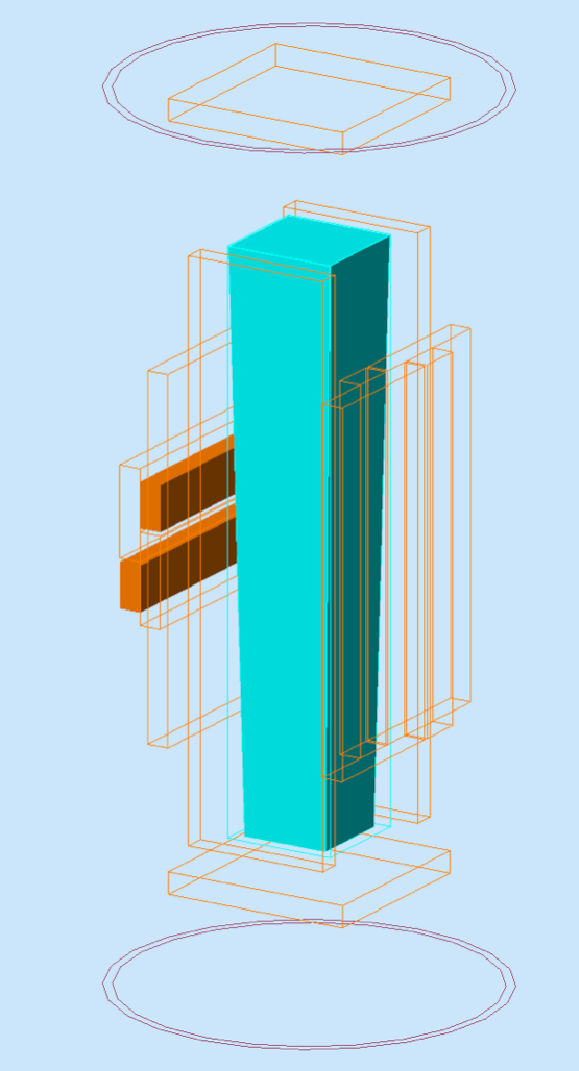
\includegraphics[width=2.9cm]{figs/gemc-3d1.pdf}  
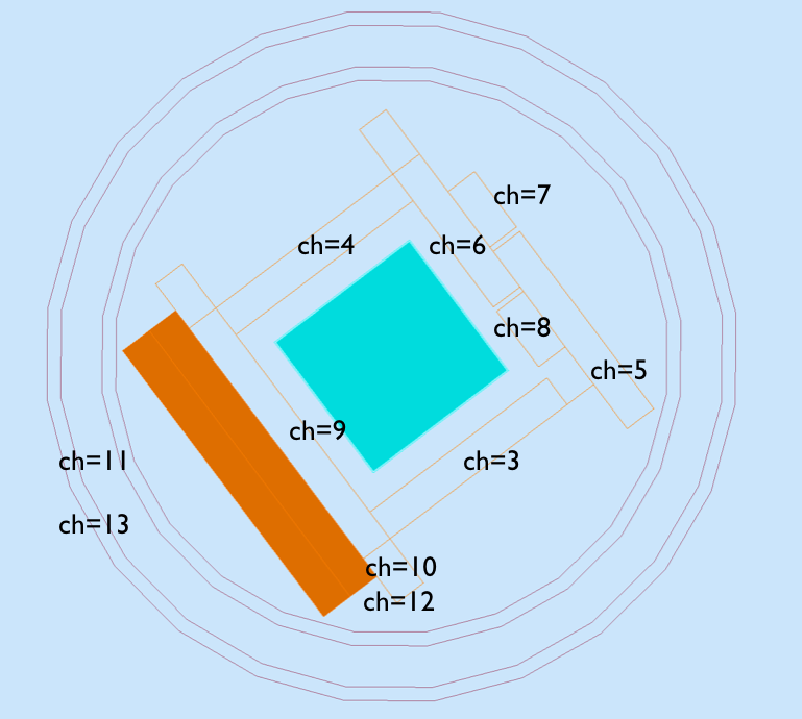
\includegraphics[width=6.0cm]{figs/gemc-3d2.pdf}  
\caption{The GEMC  implementation of the BDX-Hodo detector.}
\label{fig:det-gemc}
\end{figure}


The  detector geometry as well as the realistic response of the CsI(Tl) crystal and plastic scintillators have been implemented in GEMC (see  Appendix B.2 of PR-16-001~\cite{bdx-proposal} for details about the crystal and plastic scintillator response parametrisation). 
Figure~\ref{pic:det-gemc} shows the BDX-Hodo implementation in GEMC. 
We assumed a detection threshold of 10 phe ( in the scintillators and 100 phe in the crystal corresponding to 400 keV and 2 MeV of deposited energy respectively (MIPs release $\sim50$ phe / 2 MeV and 1670 phe /32 MeV  respectively). 



\clearpage
\section{Results}\label{sec:results}

Muons and neutrons were produced by the electron beam interaction with the beam-dump and propagated in the region of interest as described in  Sec.~\ref{sec:sampling}.


\subsubsection{Muons}
Fig.~\ref{fig:mu-comp} shows the muon flux  as obtained by GEMC and FLUKA starting from the electron/beam-dump interaction and as generated at high statistics by the custom muon generator in the  three locations of interest. Results are reported for muons generated at high statistic by the custom $\mu$ event generator and propagated using GEMC (green points in the figure).
The number of event generating at the dump correspond to  (1.2 $\pm$0.1) 10$^{12}$ EOT that correspond to a  0.2 uA 
\begin{figure}[h!] 
\center
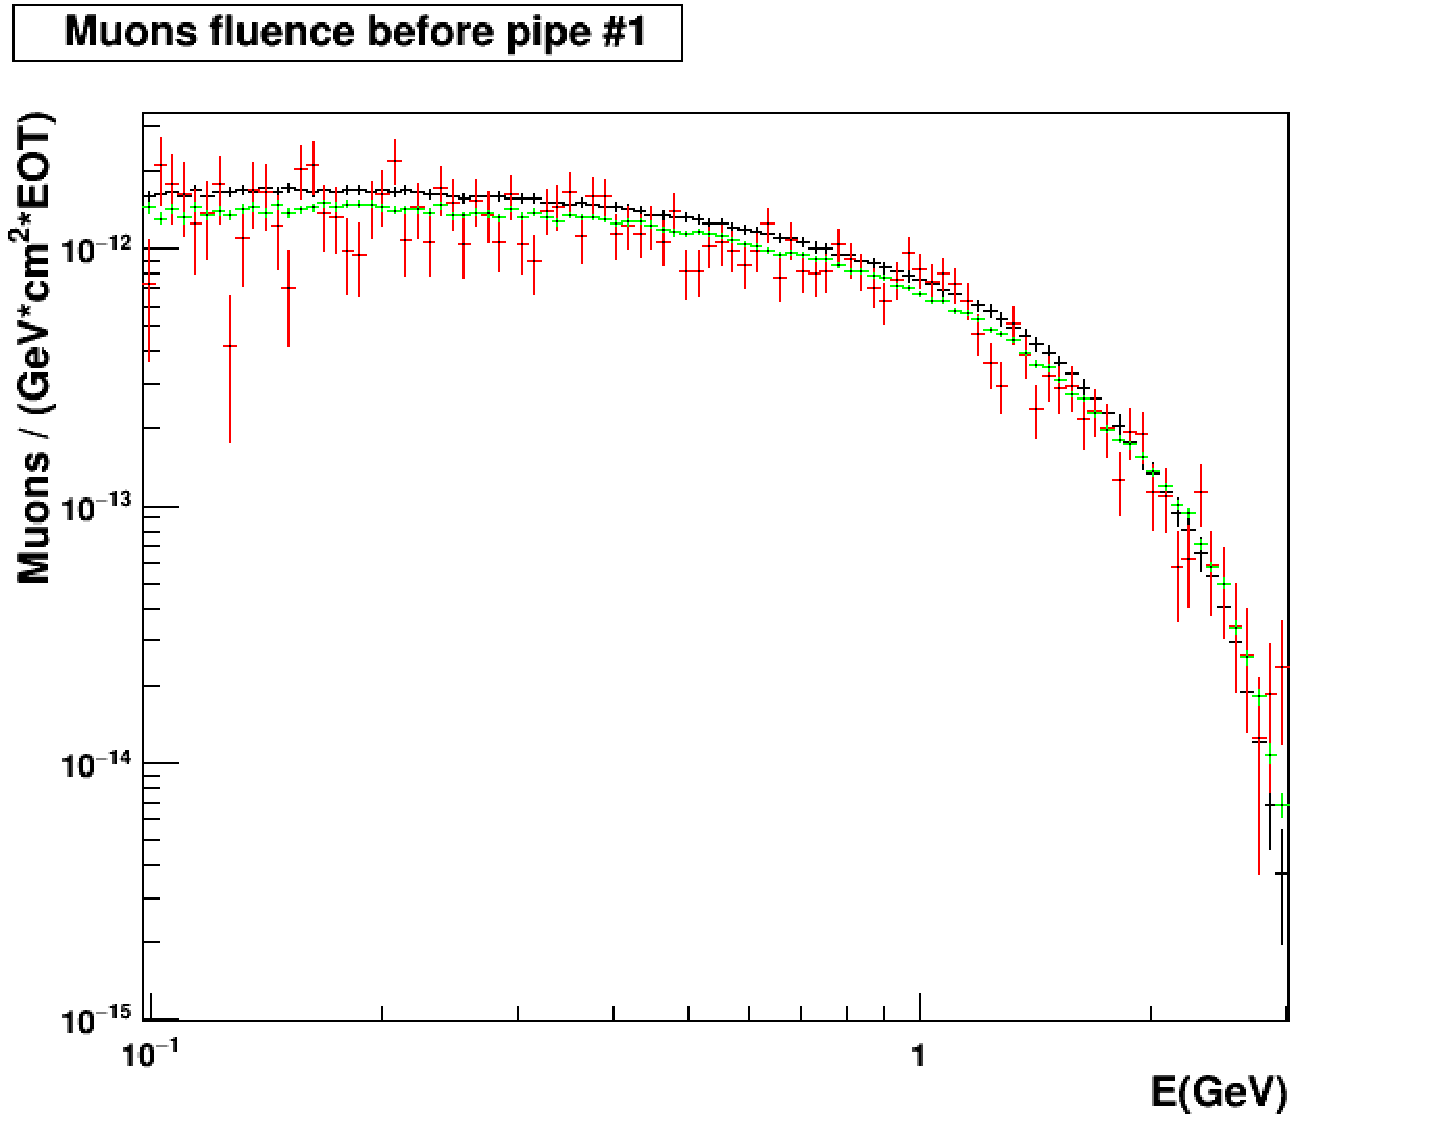
\includegraphics[width=4.7cm]{figs/comparisonMuonsPipe1_1D.pdf}
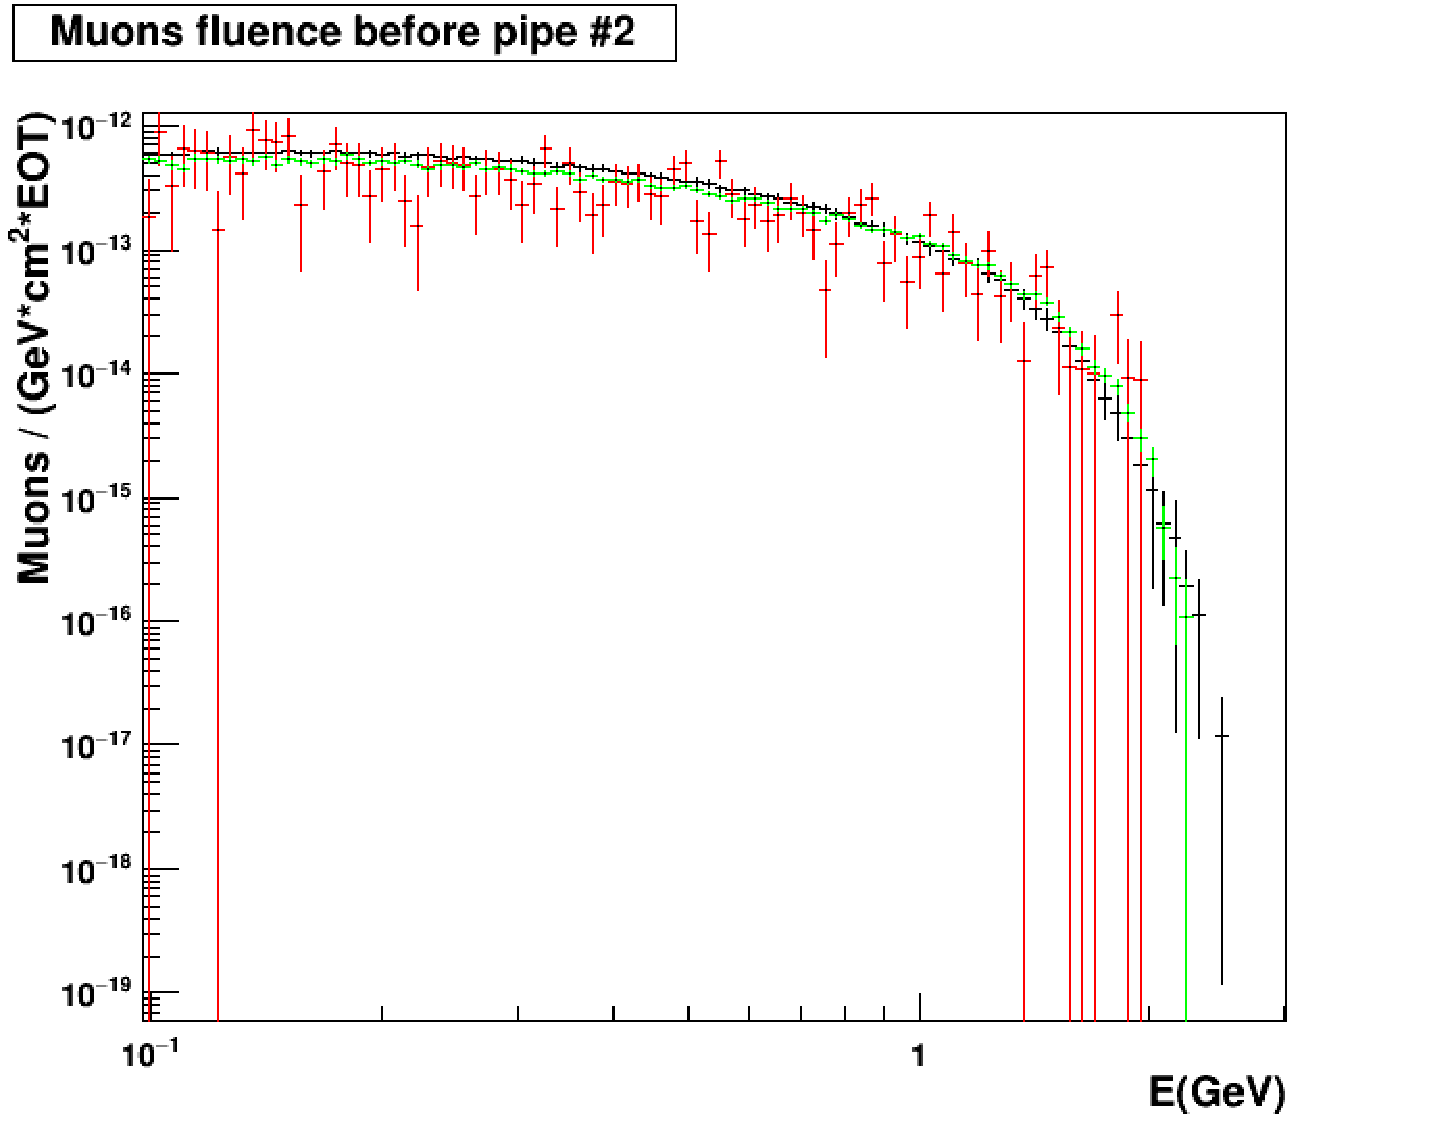
\includegraphics[width=4.7cm]{figs/comparisonMuonsPipe2_1D.pdf}
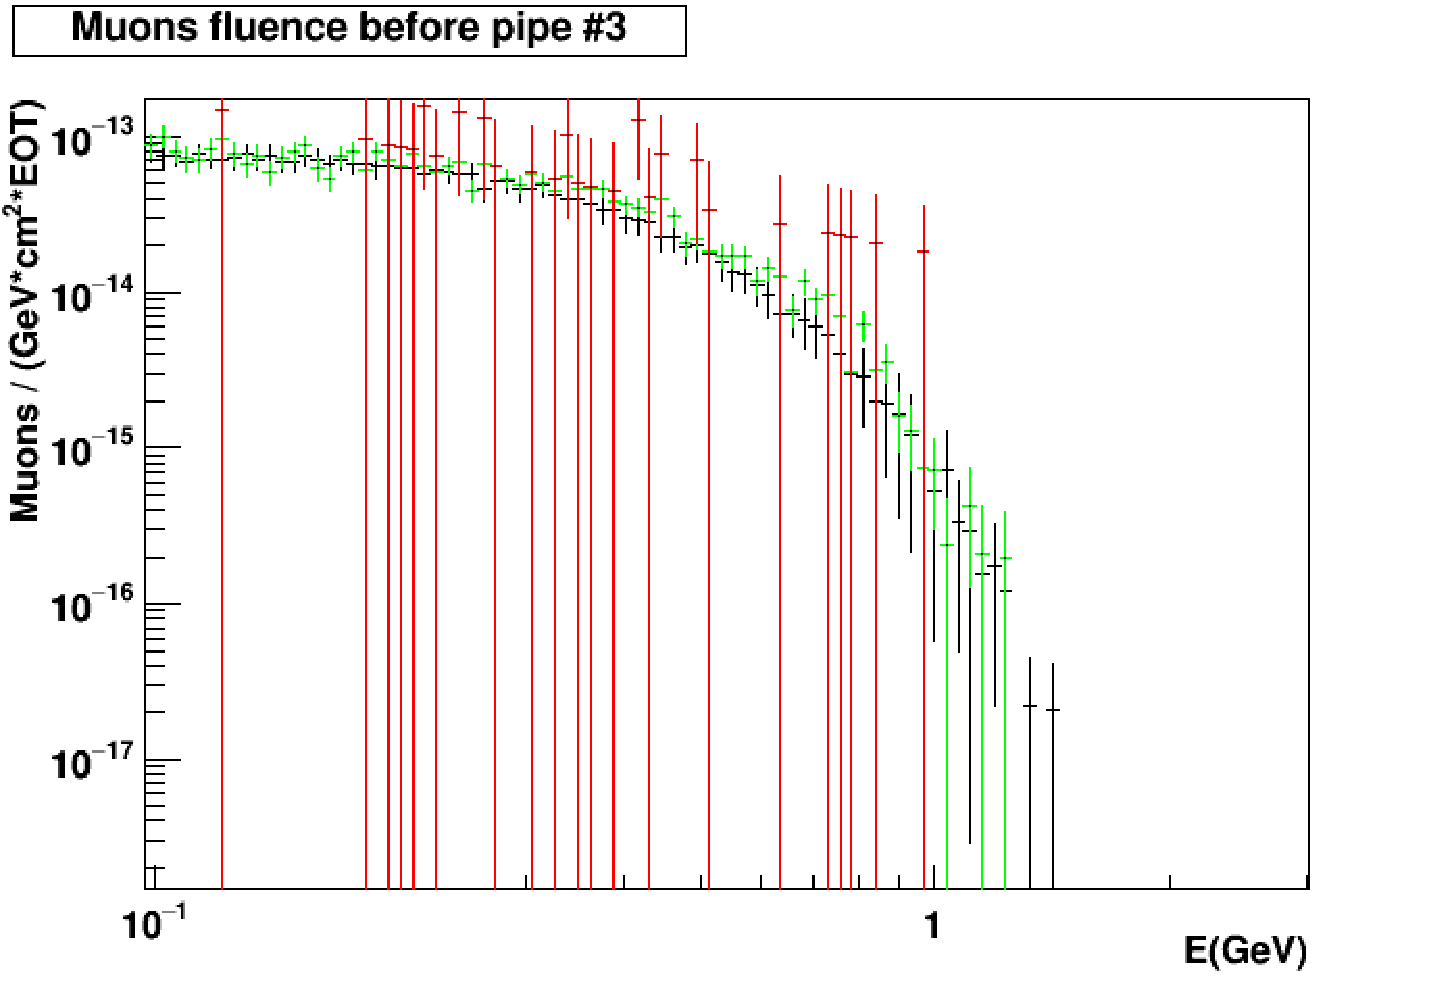
\includegraphics[width=5.5cm]{figs/comparisonMuonsPipe3_1D.pdf}
\caption{Muons energy spectra at the three locations of interest. Beam/dump interaction using  FLUKA (black), GEMC (red) and the high statistic custom $\mu$ event generator with GEMC propagation (green).}
\label{fig:mu-comp}
\end{figure}
\subsubsection{Beam-related background}



Fig.~\ref{fig:nu-comp} shows the neutron flux  as obtained by  FLUKA starting from the electron/beam-dump interaction  in the  three locations of interest. 
\begin{figure}[h!] 
\center
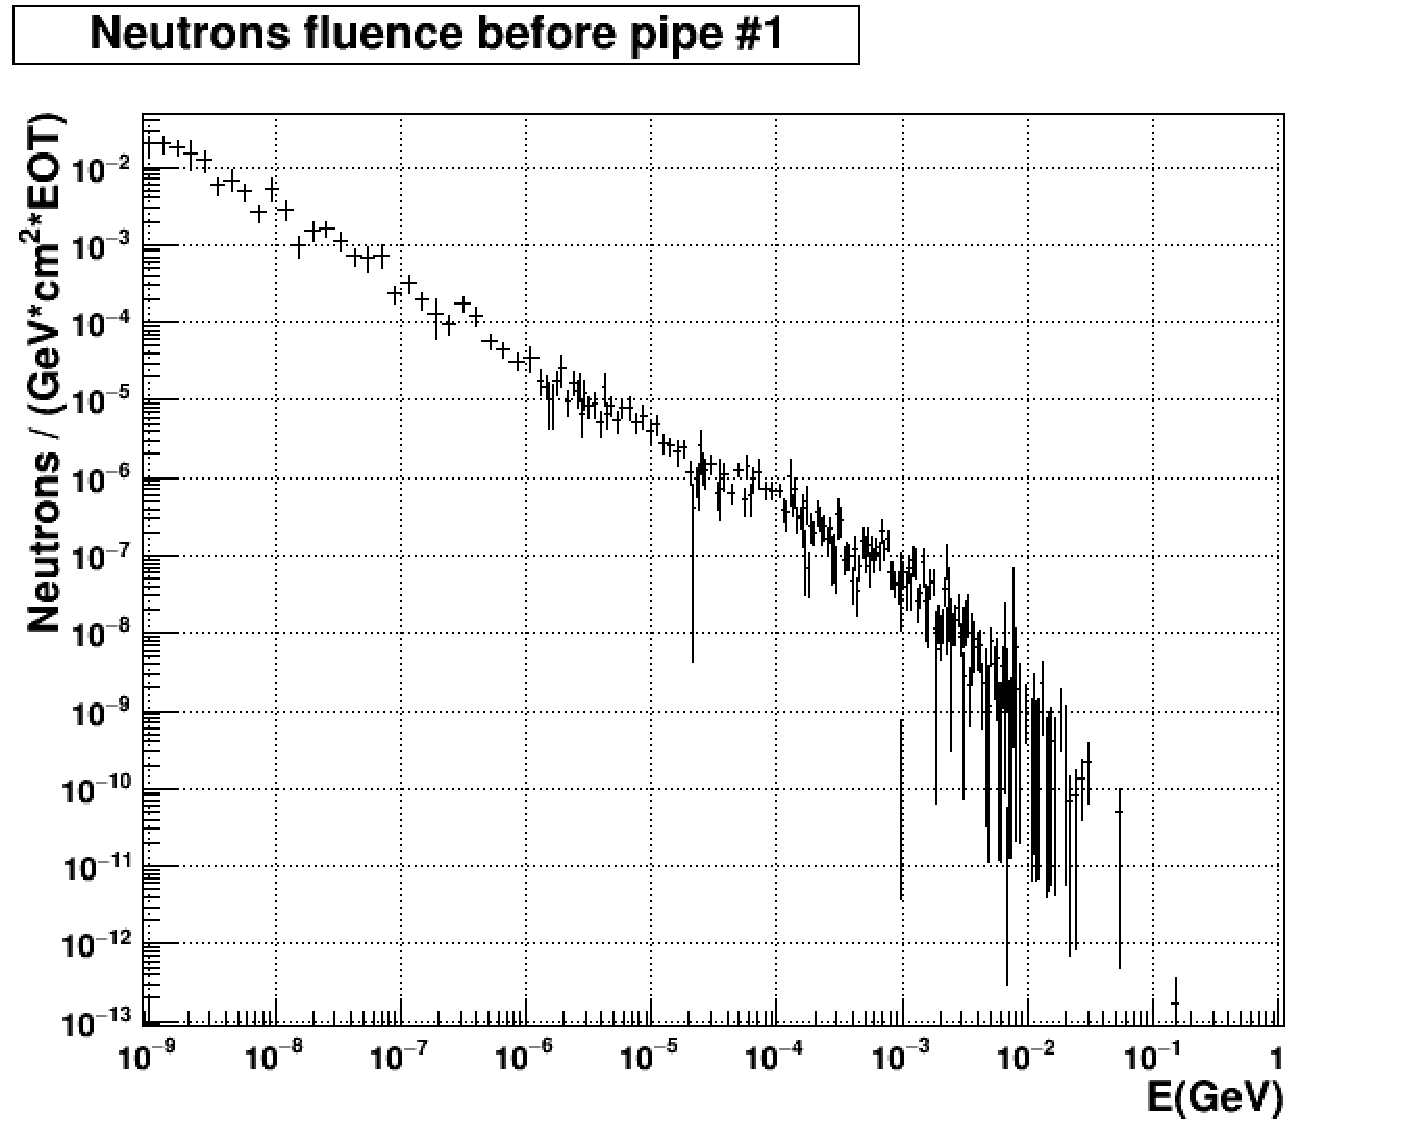
\includegraphics[width=4.7cm]{figs/NeutronsPipe1_1D.pdf}
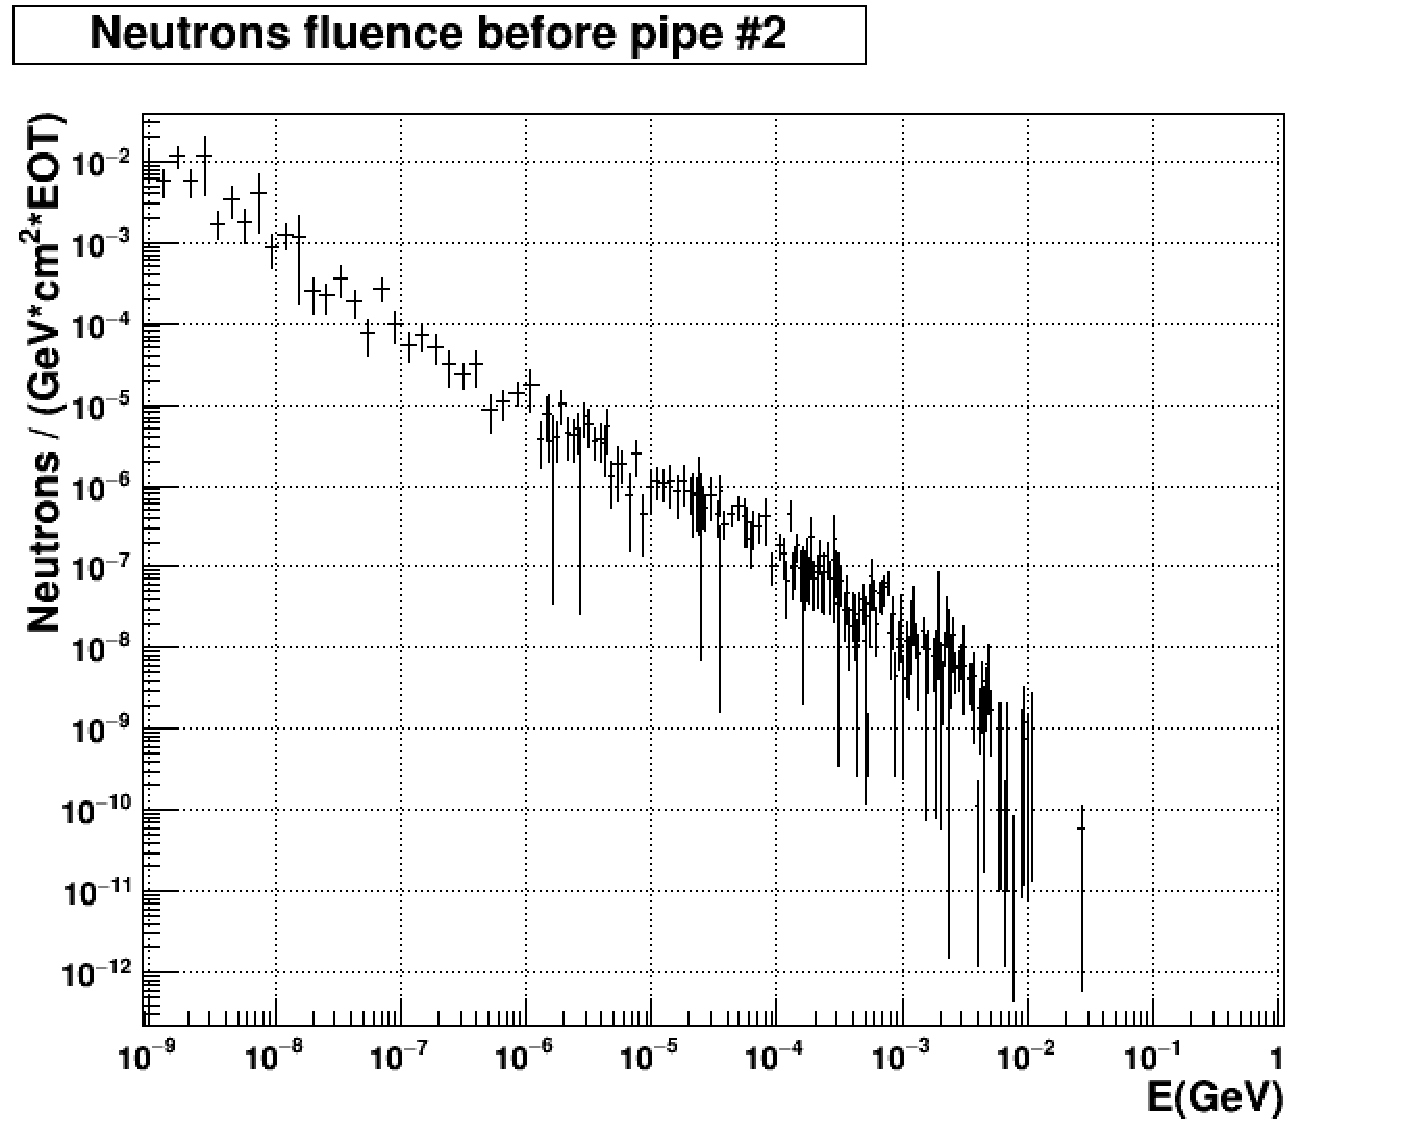
\includegraphics[width=4.7cm]{figs/NeutronsPipe2_1D.pdf}
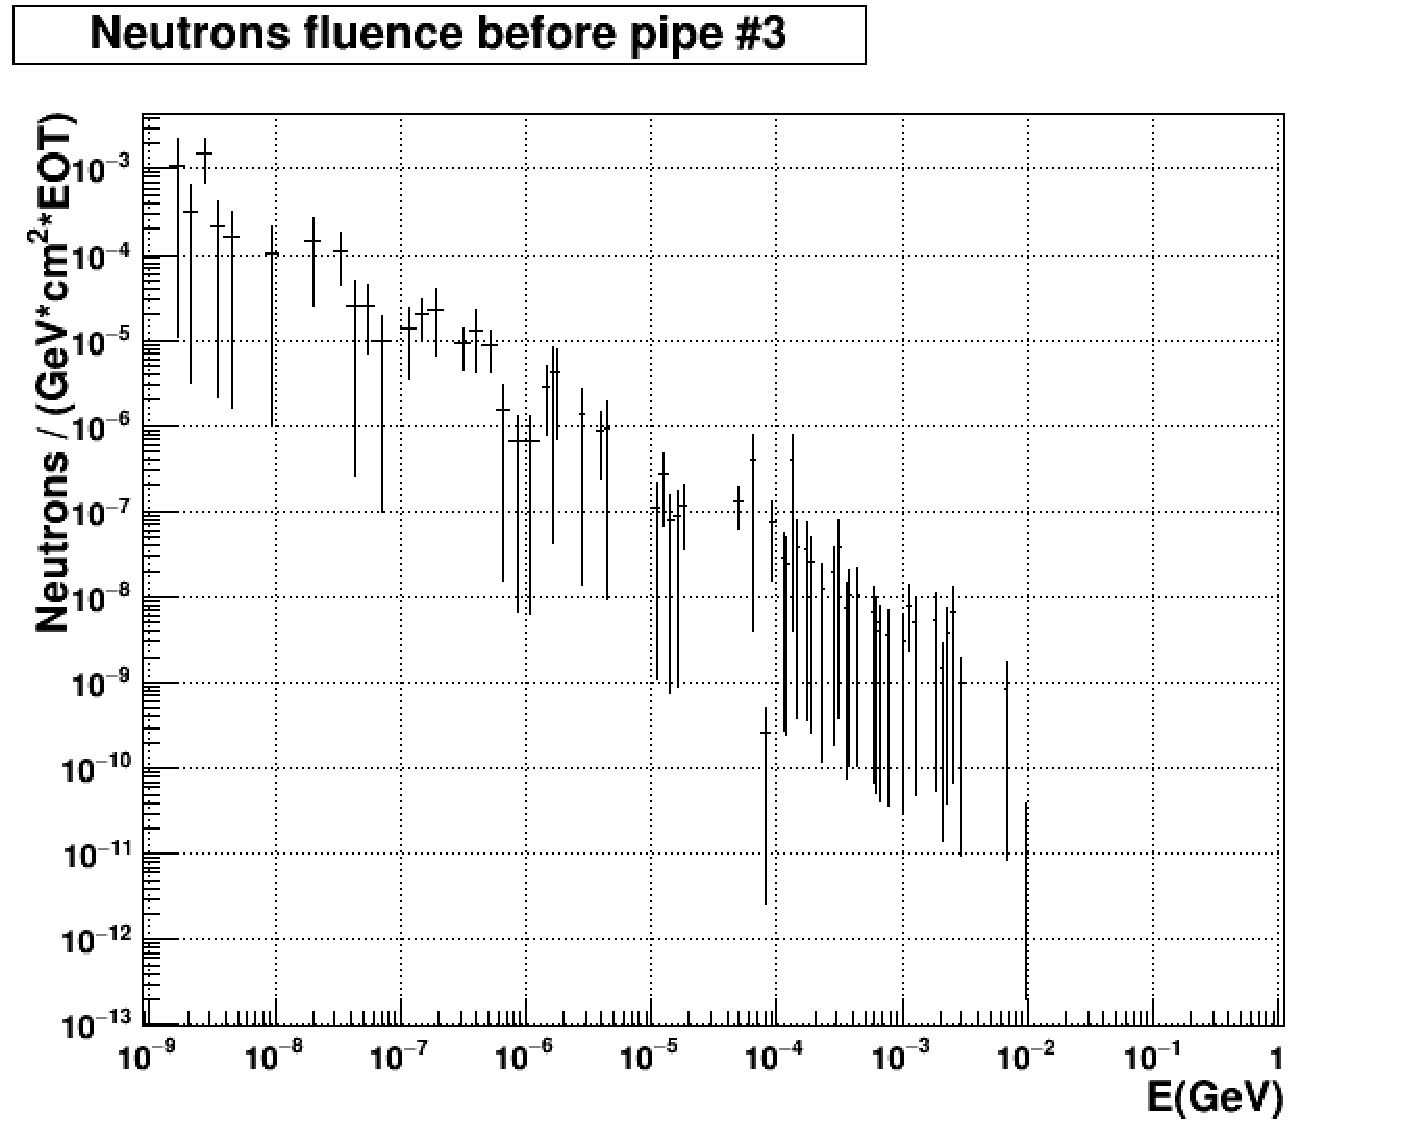
\includegraphics[width=5.5cm]{figs/NeutronsPipe3_1D.pdf}
\caption {Neutron energy spectra at the three locations of interest. Spectra are obtained from electron beam interaction with the beam-dump using FLUKA.}
\label{fig:nu-comp}
\end{figure}


\subsubsection{Cosmic background}

\subsection{The proposed test}


\clearpage
\section{Appendix}
\label{sec:appx}
\subsection{Cost estimates}
\subsection{Work-plan, time-plan, ...}
\clearpage
\clearpage

\newpage

%\nocite{*}
\bibliographystyle{unsrt}                                                                              
\bibliography{BDX-mutest-bib}

\end{document}
